\documentclass[12pt,a4paper]{article}
\usepackage[spanish,es-tabla]{babel}
\usepackage[utf8]{inputenc}
\usepackage{amsmath,amssymb,amsfonts}
\usepackage{graphicx}
\usepackage{geometry}
\usepackage{hyperref}
\usepackage{xcolor}
\usepackage{microtype}
\usepackage{csquotes}
\usepackage{setspace}
\usepackage{booktabs}
\usepackage{enumitem}
\usepackage{tabularx}
\usepackage{float}
\usepackage{xltabular}

\geometry{top=2.5cm, bottom=2.5cm, left=2.5cm, right=2.5cm}
\onehalfspacing

% Directorios de búsqueda de figuras generadas por el pipeline experimental
\graphicspath{{../../resultados/figuras/}{../../Archivos/images/}{../../resultados/}}

\hypersetup{
    colorlinks=true,
    linkcolor=blue!80!black,
    citecolor=blue!80!black,
    urlcolor=blue!80!black,
    pdftitle={Máquinas de Soporte Vectorial para la Predicción Temprana de Deserción Estudiantil Universitaria},
    pdfauthor={Sara López Chavarro, Nicolás Figueroa Salgado, Arnold Santiago Torres Anzola}
}

\begin{document}

\begin{titlepage}
    \hypersetup{pageanchor=false}
    \centering
    \vspace*{1.0cm}
    
    {\Large \textbf{UNIVERSIDAD EXTERNADO DE COLOMBIA}}\\[0.35cm]
    {\large \textbf{DEPARTAMENTO DE MATEMÁTICAS}}\\[0.25cm]
    {\large \textbf{PROGRAMA DE PREGRADO EN CIENCIA DE DATOS}}\\[2.0cm]
    
    \rule{\linewidth}{0.6mm}\\[0.6cm]
    {\Large \bfseries Máquinas de Soporte Vectorial para la Predicción Temprana de Deserción Estudiantil Universitaria bajo Diferentes Métodos de Normalización}\\[0.5cm]
    {\large \textit{Propuesta de Adaptación y Réplica Experimental con Metodología SPADIES 3.0}}\\[0.5cm]
    \rule{\linewidth}{0.6mm}\\[1.5cm]
    
    {\large \textbf{Machine Learning II}}\\[2.0cm]
    
    \begin{minipage}{0.85\textwidth}
        \centering
        \textbf{\large Integrantes / Investigadores:}\\[0.4cm]
        {\large \textbf{Sara López Chavarro}}\\[0.25cm]
        {\large \textbf{Nicolás Figueroa Salgado}}\\[0.25cm]
        {\large \textbf{Arnold Santiago Torres Anzola}}
    \end{minipage}\\[2.5cm]
    
    \vfill
    
    {\large Bogotá D.C., Colombia}\\[0.2cm]
    {\large 2026}
\end{titlepage}

\hypersetup{pageanchor=true}
\newpage
\pagenumbering{arabic}

\section{El problema planteado en el artículo}

El artículo base seleccionado, titulado \textit{``Support Vector Machine for Predicting Student Dropout Under Different Normalization Methods''} \cite{boteju2024}, aborda la problemática de la deserción y el retraso en la graduación en la educación superior. Este fenómeno genera costos económicos y psicológicos significativos tanto para los estudiantes (endeudamiento y pérdida de tiempo) como para las instituciones (pérdida de eficiencia y recursos). La detección temprana de estudiantes en riesgo es un desafío complejo debido a la influencia multifactorial de variables socioeconómicas, demográficas y académicas \cite[pág.~8633]{boteju2024}.

\section{El método usado en el artículo}

El estudio implementa Máquinas de Soporte Vectorial (SVM) para clasificar el estado final del estudiante. Su núcleo metodológico radica en evaluar el impacto de técnicas diferentes de preprocesamiento y normalización de datos (como \texttt{StandardScaler}, \texttt{MinMaxScaler}, \texttt{OneHotEncoder}, \texttt{QuantileTransformer}, entre otros) sobre la capacidad predictiva del modelo \cite[pág.~8633]{boteju2024}. Validan los resultados mediante ejecuciones iterativas de 50 ensayos para garantizar estabilidad estadística \cite[pág.~8635]{boteju2024}.

\subsection{Supuestos principales del artículo}
\begin{itemize}
    \item \textbf{Relaciones no lineales:} Los datos presentan relaciones complejas que pueden ser separadas en espacios de alta dimensión mediante el uso de funciones de kernel (truco del kernel).
    \item \textbf{Sensibilidad al escalado:} La escala y la transformación de las características de entrada alteran de forma directa la posición de los hiperplanos de separación y los vectores de soporte, afectando la generalización del modelo.
    \item \textbf{Multifactorialidad:} Las variables socioeconómicas, demográficas y académicas capturan las señales latentes de riesgo de abandono escolar.
\end{itemize}

\subsection{Resultados reportados y limitaciones}
\begin{itemize}
    \item \textbf{Resultados:} Se demostró que el preprocesamiento es crítico; los métodos escalados superan ampliamente a los modelos sin normalización.
    \item \textbf{Limitaciones:} El estudio se limita a un dataset específico de la UC Irvine de 4,424 registros y explora un conjunto cerrado de transformaciones, dejando abierta la discusión sobre cómo se comportan estas técnicas frente a clases altamente desbalanceadas en contextos institucionales específicos de América Latina.
\end{itemize}

\section{Planteamiento del Problema en un Contexto Local}

\subsection{Pregunta de investigación}
¿Es posible predecir de manera temprana el riesgo de deserción académica en estudiantes universitarios de pregrado en Colombia mediante un flujo robusto de Machine Learning basado en SVM, optimizando el rendimiento predictivo a través de técnicas avanzadas de normalización de datos y proveyendo interpretabilidad institucional a las decisiones del modelo?

\subsection{Tipo de tarea}
Problema de clasificación multiclase con 3 categorías mutuamente excluyentes conforme a los estándares oficiales del Ministerio de Educación Nacional de Colombia (MEN):
\begin{itemize}
    \item \textbf{Graduado:} Estudiante que culmina su plan de estudios exitosamente.
    \item \textbf{En curso:} Estudiante activo que continúa su proceso formativo regular.
    \item \textbf{Desertor:} Estudiante que abandona formal o informalmente el programa.
\end{itemize}

Para mayor precisión analítica, se adoptan las definiciones institucionales de abandono:
\begin{description}[style=multiline, leftmargin=3.5cm]
    \item[Abandono formal:] Ocurre cuando el estudiante realiza un trámite administrativo e institucional de retiro oficial (cancelación de matrícula, solicitud formal de retiro).
    \item[Abandono informal (silencioso):] Ocurre cuando el estudiante simplemente deja de asistir a clases, abandona las evaluaciones y no renueva matrícula, sin notificar a la universidad. Este abandono suele ser tardíamente detectado sin herramientas predictivas.
\end{description}

\section{Estrategia de Datos (Fundamentación SPADIES 3.0)}

Se adoptó el marco conceptual y metodológico del Sistema para la Prevención y Análisis de la Deserción en las Instituciones de Educación Superior (SPADIES 3.0) del Ministerio de Educación Nacional de Colombia \cite{mineducacion2024} y los desarrollos del Sistema de Alerta Temprana (SAT-DE) \cite{penapico2024}.

\subsection{Estructura del Dataset}
El conjunto de datos comprende \textbf{11,500 registros de estudiantes} y \textbf{21 características predictoras} distribuidas en dimensiones académicas, socioeconómicas y demográficas. La variable objetivo multiclase fue formulada mediante el Índice de Riesgo Ponderado SPADIES ($R_i \in [0.0, 8.0]$), asignando condición de deserción a estudiantes con $R_i \ge 3.5$, graduación para aquellos con semestre mayor a la duración nominal y promedio acumulado $\ge 3.2$, y permanencia activa (en curso) para los demás casos.

\begin{table}[htbp]
\centering
\caption{Variables predictoras cuantitativas y cualitativas del dataset ($n=11,500$)}
\label{tab:variables_resumen}
\small
\begin{tabularx}{\textwidth}{l l X}
\toprule
\textbf{Variable} & \textbf{Tipo} & \textbf{Descripción Conceptual} \\
\midrule
\texttt{edad\_ingreso} & Numérica & Edad biológica al ingresar al programa universitario (15--35 años). \\
\texttt{promedio\_academico} & Numérica & Promedio acumulado de calificaciones en escala nacional (0.0--5.0). \\
\texttt{materias\_reprobadas} & Numérica & Conteo acumulado de asignaturas perdidas. \\
\texttt{distancia\_hogar\_ies\_km} & Numérica & Distancia física entre la vivienda y el campus (marcada asimetría). \\
\texttt{puntaje\_icfes\_percentil} & Numérica & Percentil nacional en las pruebas de Estado Saber 11 (1--100). \\
\texttt{semestre\_cursado} & Numérica & Nivel de avance lectivo en el plan de estudios. \\
\texttt{estrato\_socioeconomico} & Numérica & Estratificación socioeconómica del hogar (1 al 6). \\
\texttt{trabaja\_mientras\_estudia} & Binaria & Indicador de actividad laboral simultánea (0: No, 1: Sí). \\
\texttt{beneficiario\_icetex} & Binaria & Apoyo financiero mediante crédito estatal educativo (0: No, 1: Sí). \\
\texttt{beneficiario\_beca} & Binaria & Subsidio o beca institucional de matrícula (0: No, 1: Sí). \\
\texttt{sexo}, \texttt{zona\_residencia} & Categórica & Datos sociodemográficos básicos (Hombre/Mujer, Urbana/Rural). \\
\texttt{sector\_ies}, \texttt{metodologia} & Categórica & Carácter jurídico (Oficial/Privado) y modalidad (Presencial/Virtual). \\
\texttt{nivel\_formacion} & Categórica & Nivel académico (Técnico, Tecnológico, Universitario). \\
\bottomrule
\end{tabularx}
\end{table}

\section{Análisis Exploratorio Visual de Datos (EDA)}

En lugar de limitarse a tablas numéricas, el análisis exploratorio se fundamenta en la interpretación visual del comportamiento de las características. La Figura \ref{fig:eda_distribucion} presenta la composición global de las cohortes y el contraste entre correlaciones lineales y no lineales.

\begin{figure}[htbp]
\centering
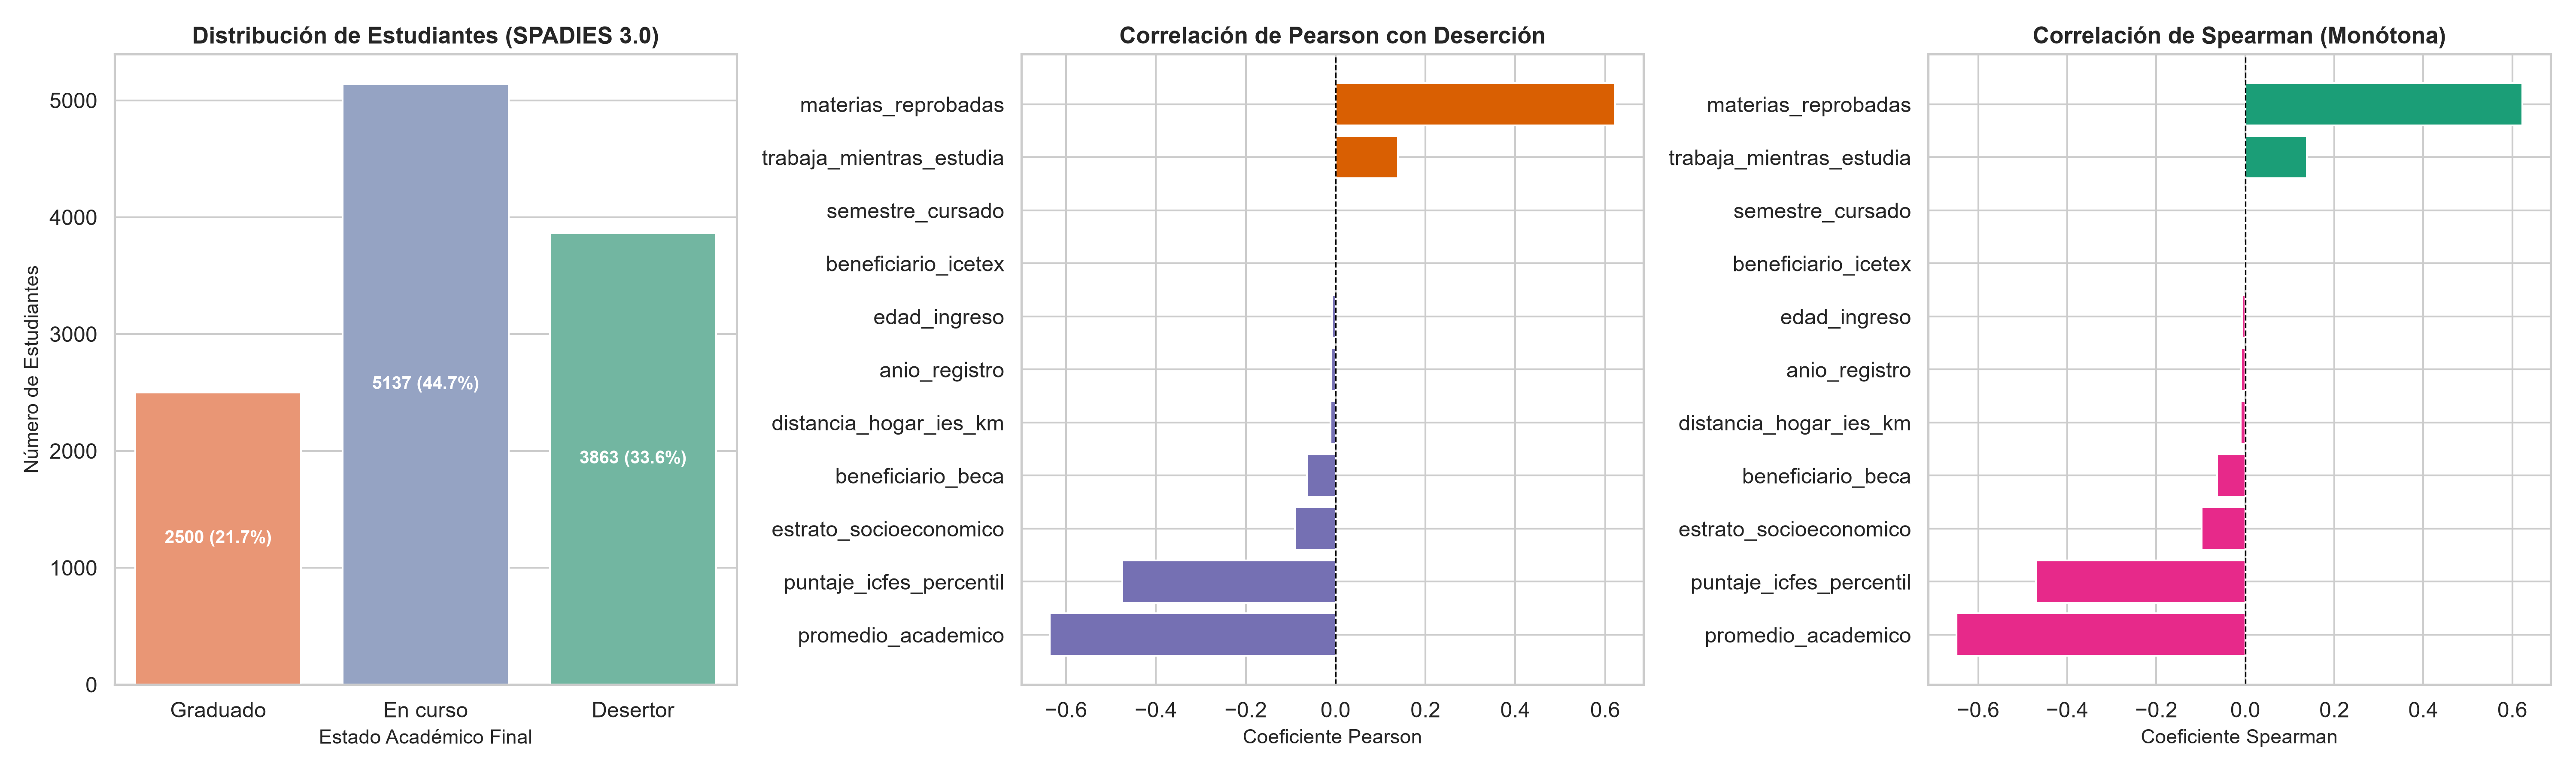
\includegraphics[width=0.98\textwidth]{eda_distribucion_correlaciones.png}
\caption{Distribución muestral de las clases SPADIES 3.0 (izquierda) y contraste entre la correlación lineal de Pearson (centro) y la correlación monótona de Spearman (derecha) frente al riesgo de deserción.}
\label{fig:eda_distribucion}
\end{figure}

\subsection{Interpretación de la Figura \ref{fig:eda_distribucion}}
\begin{enumerate}
    \item \textbf{Composición Muestral y Desbalance Controlado}: La población estudiantil presenta un $44.7\%$ de estudiantes activos (\texttt{En curso}, 5,137 registros), un $33.6\%$ en condición de abandono (\texttt{Desertor}, 3,863 registros) y un $21.7\%$ titulados (\texttt{Graduado}, 2,500 registros). Esta proporción refleja fielmente las tasas de retención observadas en la educación superior en Colombia.
    \item \textbf{No Linealidad del Fenómeno (Pearson vs. Spearman)}: Al comparar las correlaciones lineales con las monótonas, se evidencia que variables críticas como el \texttt{promedio\_academico} y las \texttt{materias\_reprobadas} exhiben magnitudes de correlación significativamente mayores bajo el coeficiente de Spearman. Esto demuestra que la deserción no sigue un deterioro lineal continuo, sino un comportamiento de umbral abrupto: cuando el promedio desciende de un nivel crítico (3.0), la probabilidad de abandono se dispara. Esta no linealidad justifica plenamente el empleo de Máquinas de Soporte Vectorial con kernel RBF frente a regresiones lineales tradicionales.
\end{enumerate}

\subsection{El Valle Académico de la Deserción}
La Figura \ref{fig:eda_variables_clave} contrasta la dispersión de las dos variables académicas más influyentes entre los tres estados de los estudiantes.

\begin{figure}[htbp]
\centering
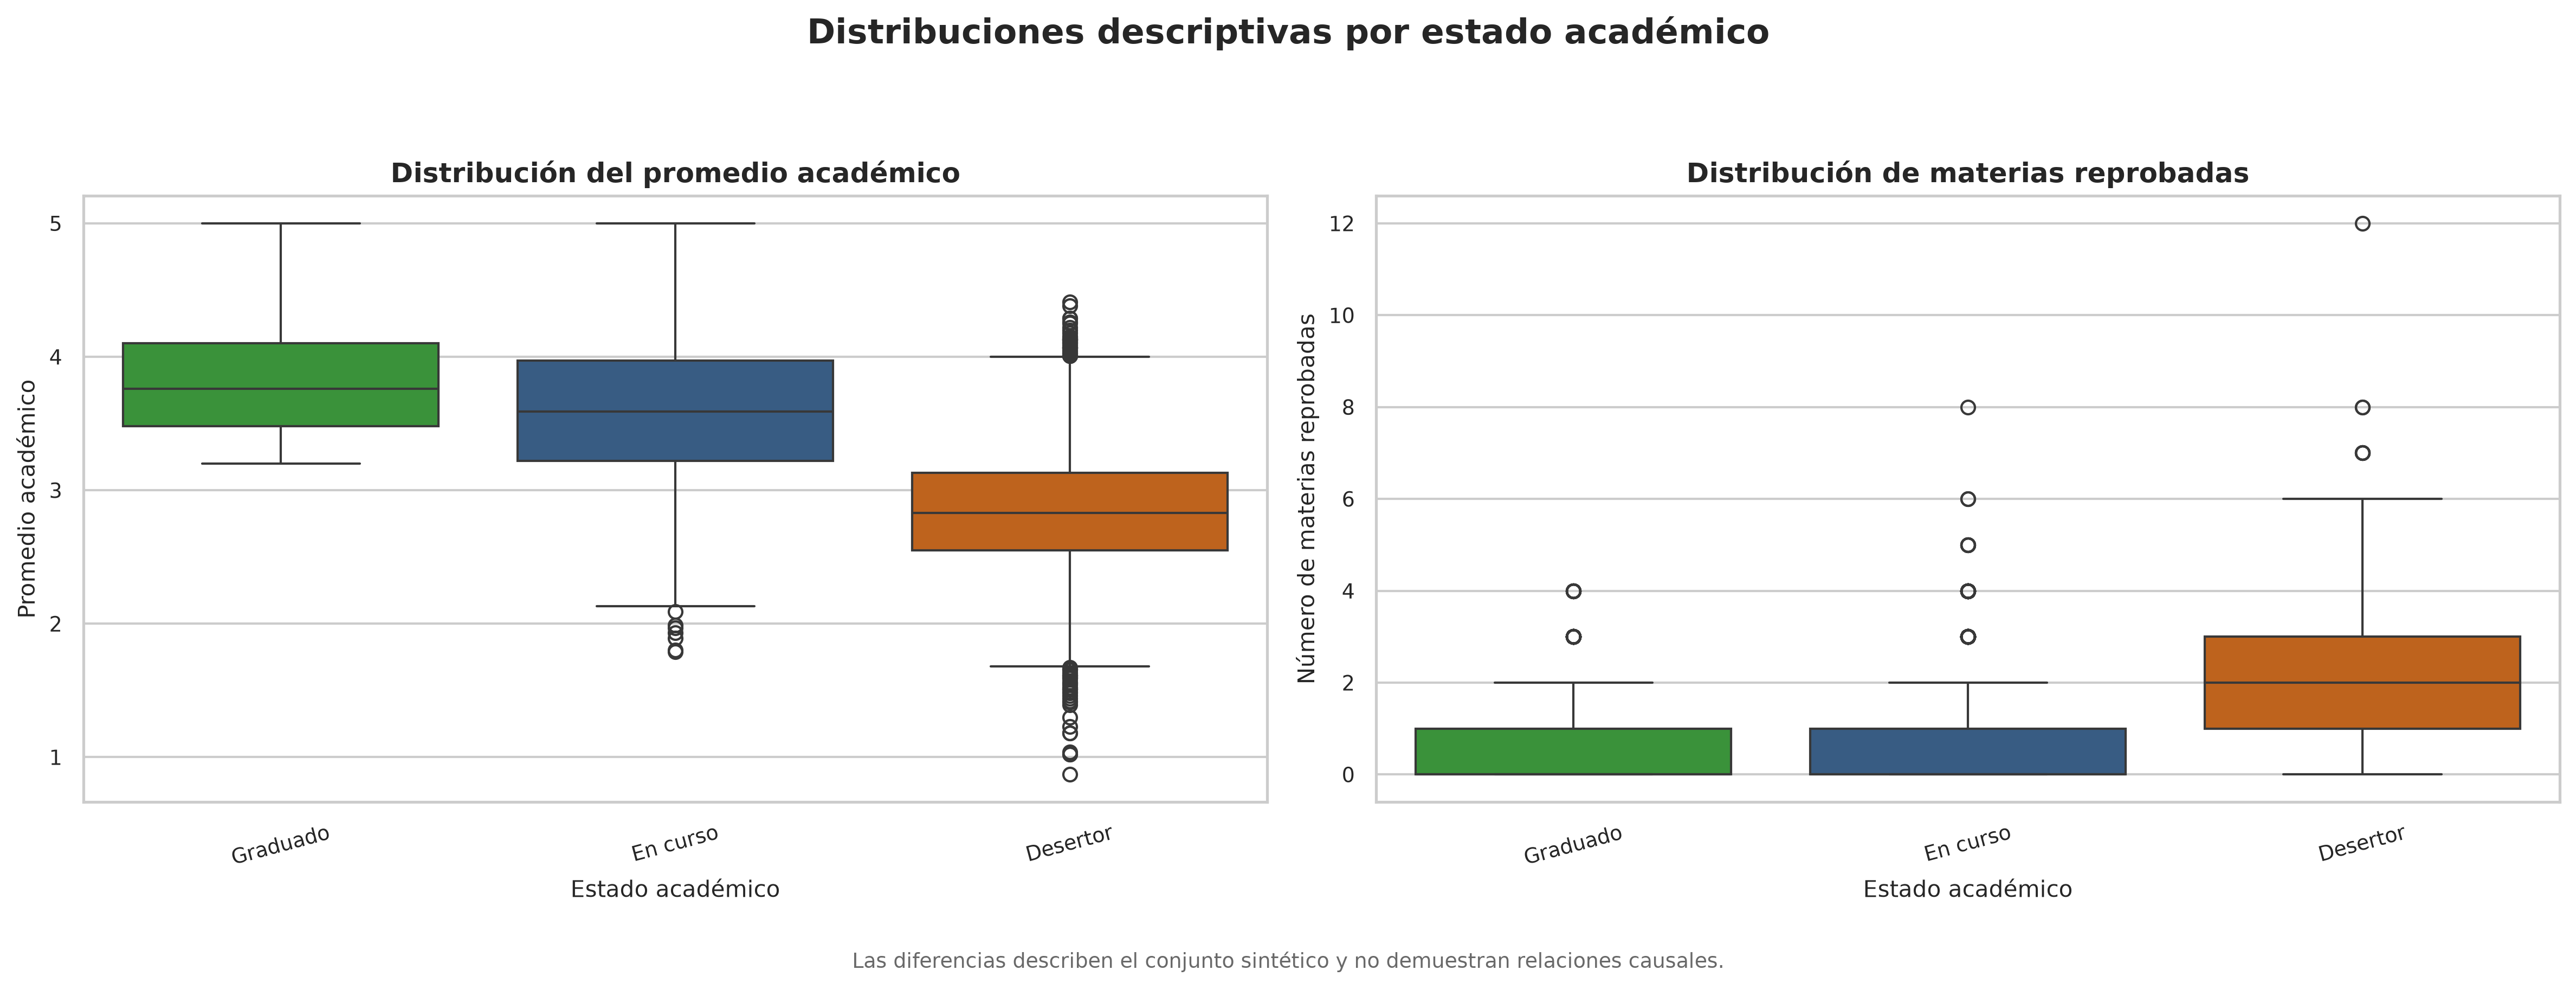
\includegraphics[width=0.90\textwidth]{eda_variables_clave.png}
\caption{Diagramas de caja (\textit{Boxplots}) del promedio acumulado (izquierda) y materias reprobadas (derecha) según el estado del estudiante.}
\label{fig:eda_variables_clave}
\end{figure}

Como se aprecia en la Figura \ref{fig:eda_variables_clave}, existe una separación nítida entre la población que culmina sus estudios y la que deserta:
\begin{itemize}
    \item \textbf{Promedio Académico}: Los desertores presentan una mediana marcadamente inferior ($2.70$), concentrándose por debajo del umbral de aprobación ($3.0$), en contraste con los graduados cuya mediana se sitúa en $3.90$.
    \item \textbf{Materias Reprobadas}: Mientras que los graduados y estudiantes en curso tienen una mediana de cero reprobadas, los desertores exhiben una dispersión amplia con concentración en 2 o más asignaturas perdidas, configurando el síntoma más temprano de desconexión institucional.
\end{itemize}

\section{El Impacto de la Escala y Demostración de Normalizadores}

Las Máquinas de Soporte Vectorial dependen intrínsecamente del cálculo de distancias geométricas en el espacio inducido:
\begin{equation}
K(x_i, x_j) = \exp\left(-\gamma \|x_i - x_j\|^2\right)
\end{equation}
Si una característica posee una escala numérica órdenes de magnitud superior a las demás, dominará artificialmente la norma euclidiana $\|x_i - x_j\|^2$, anulando la capacidad del clasificador para aprender de variables con menor rango pero mayor poder discriminante (como el promedio de 0 a 5).

La variable \texttt{distancia\_hogar\_ies\_km} representa el caso más severo en el dataset, al presentar una asimetría positiva extrema ($\text{Skewness} = +5.05$) con un $7.17\%$ de valores atípicos (estudiantes de regiones remotas a más de 50 km). La Figura \ref{fig:eda_efecto_escaladores} muestra empíricamente cómo reacciona esta variable ante seis métodos de transformación.

\begin{figure}[htbp]
\centering
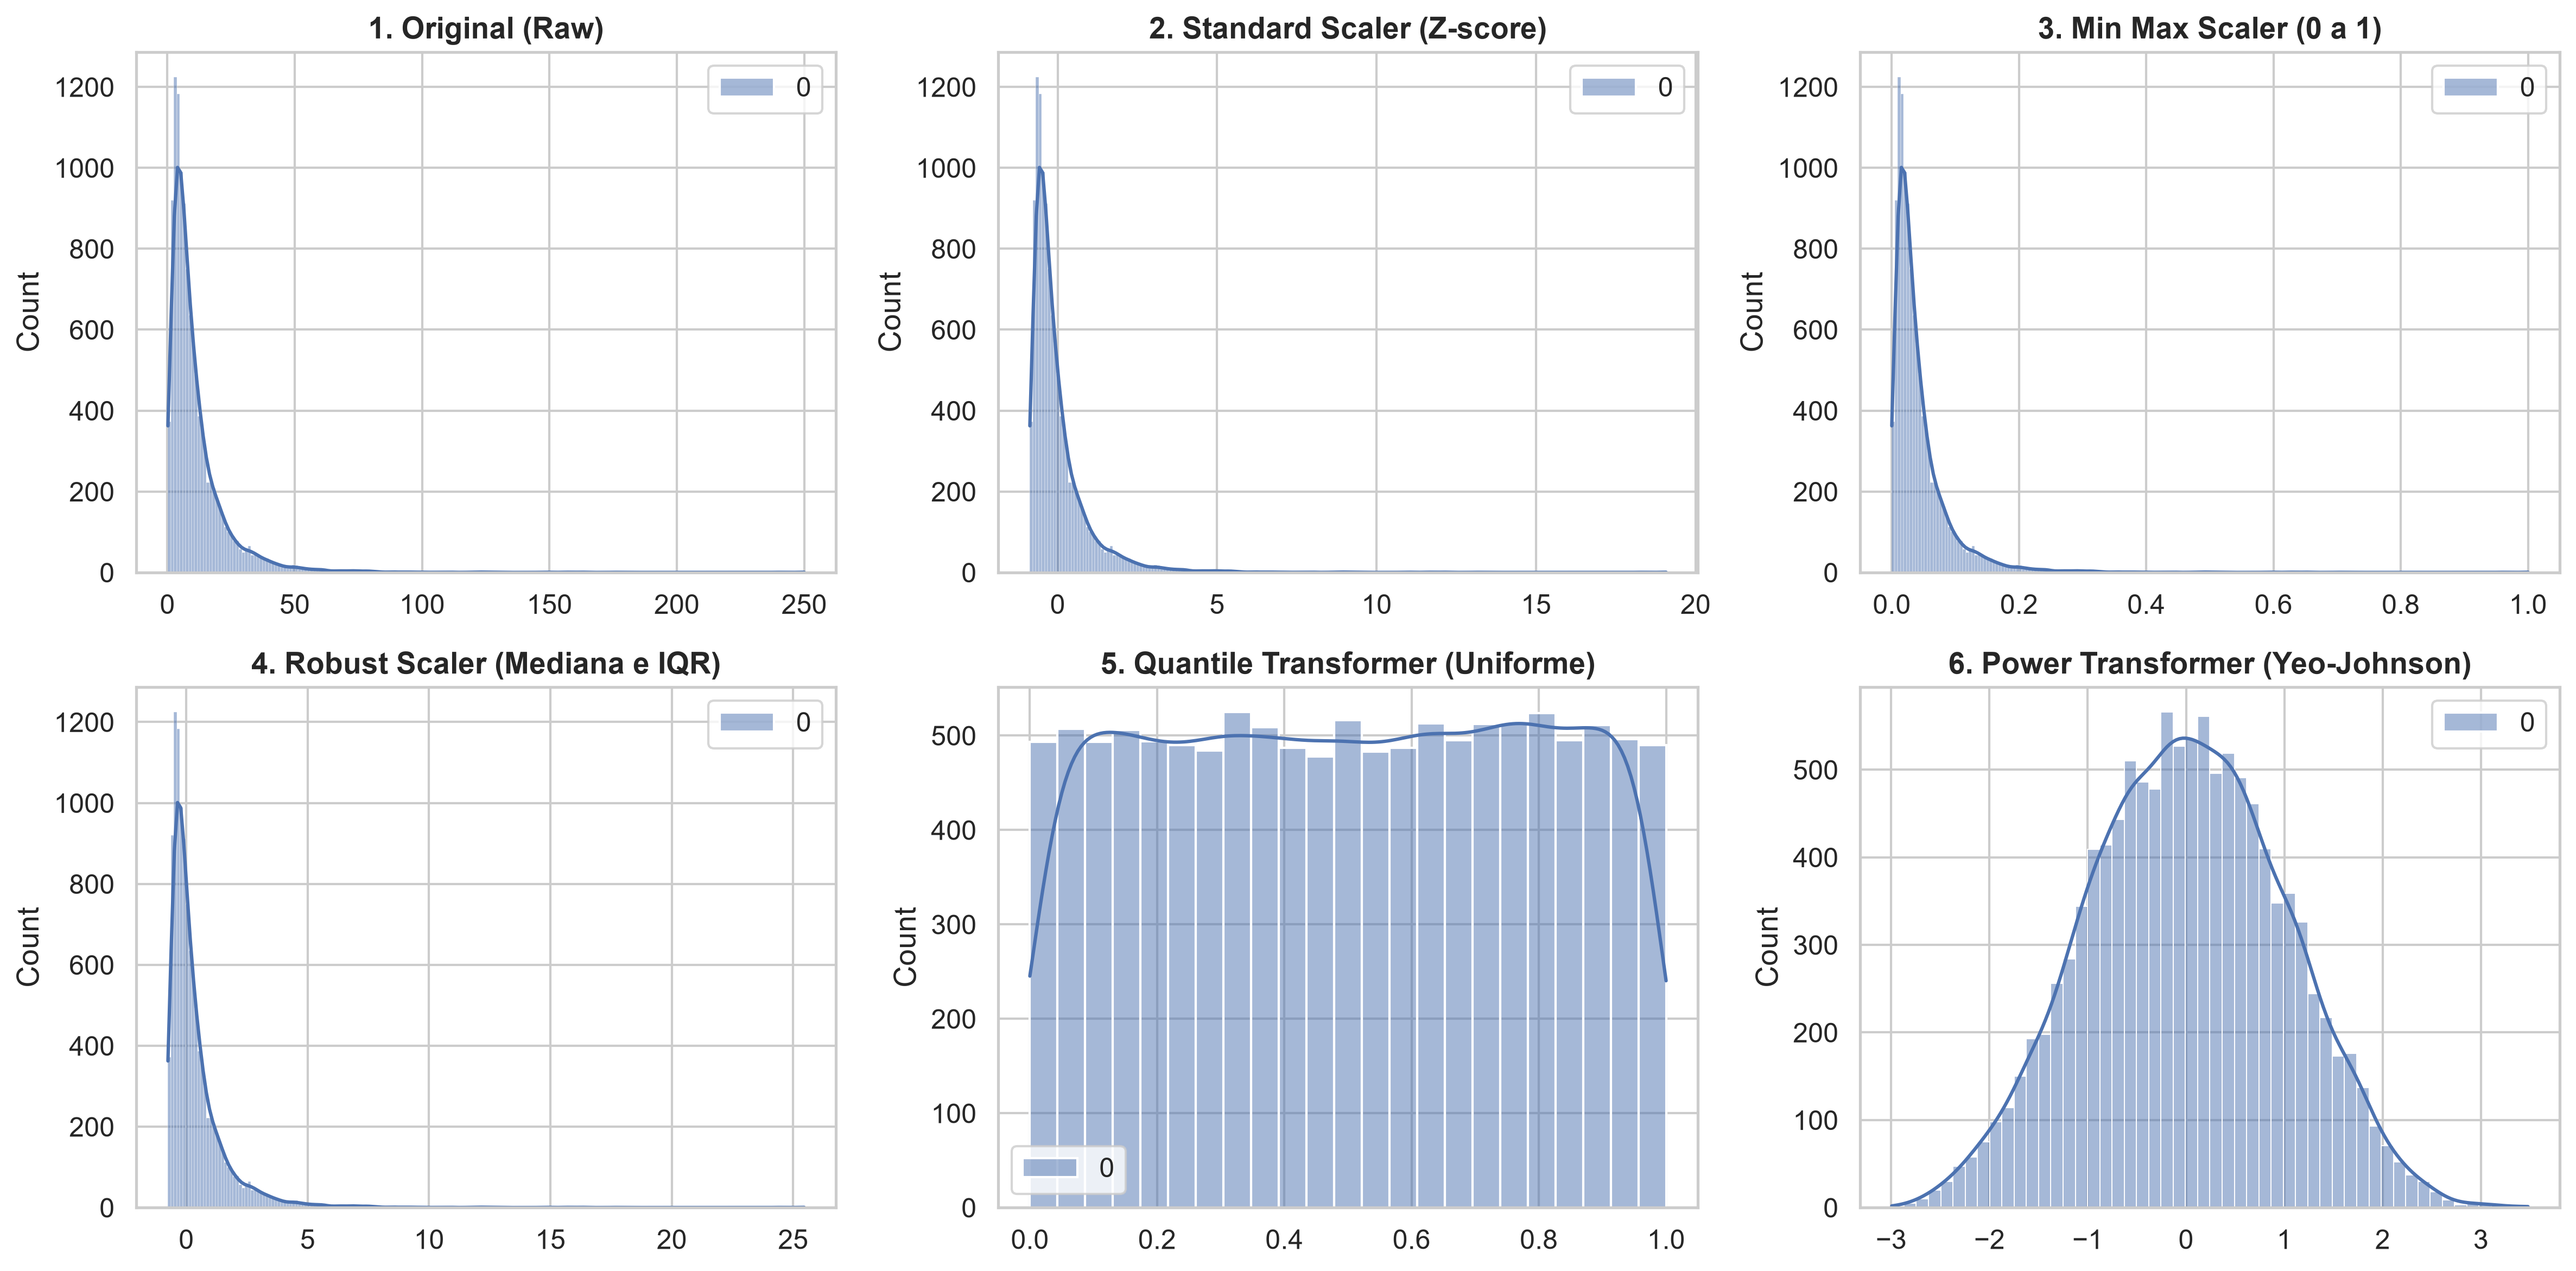
\includegraphics[width=0.98\textwidth]{eda_efecto_escaladores.png}
\caption{Demostración visual del efecto de seis transformaciones cuantitativas sobre la densidad y dispersión de la variable con asimetría positiva (\texttt{distancia\_hogar\_ies\_km}).}
\label{fig:eda_efecto_escaladores}
\end{figure}

\subsection{Interpretación Visual de los Escaladores (Figura \ref{fig:eda_efecto_escaladores})}
\begin{itemize}
    \item \textbf{1. Escala Original (Raw)}: Presenta una cola alargada hacia la derecha que colapsaría el cálculo de distancias en SVM.
    \item \textbf{2. StandardScaler}: Centra la masa en cero, pero los valores extremos se extienden hasta $Z > 10$, manteniendo cierta vulnerabilidad ante outliers.
    \item \textbf{3. MinMaxScaler}: Comprime toda la masa poblacional en un intervalo estrecho cercano a 0 debido al efecto de los valores máximos alejados.
    \item \textbf{4. RobustScaler}: Utiliza la mediana y el rango intercuartílico ($IQR$), evitando que los estudiantes de zonas rurales distorsionen la escala del 90\% restante.
    \item \textbf{5. QuantileTransformer y 6. PowerTransformer}: Logran una transformación cuasi-gaussiana y uniforme respectivamente, estabilizando la varianza y mitigando por completo el sesgo de la cola larga.
\end{itemize}

\section{Resultados Experimentales: Ranking de Normalizadores}

Para validar el impacto del escalado de forma reproducible y sin fuga de datos, se ejecutó un experimento de \textbf{50 particiones independientes} ($N=50$ \textit{trials}), entrenando 400 modelos SVM mediante \texttt{Pipeline} y \texttt{ColumnTransformer}. La Figura \ref{fig:ranking_normalizadores} resume el desempeño comparativo en $F_1$-Score Ponderado.

\begin{figure}[htbp]
\centering
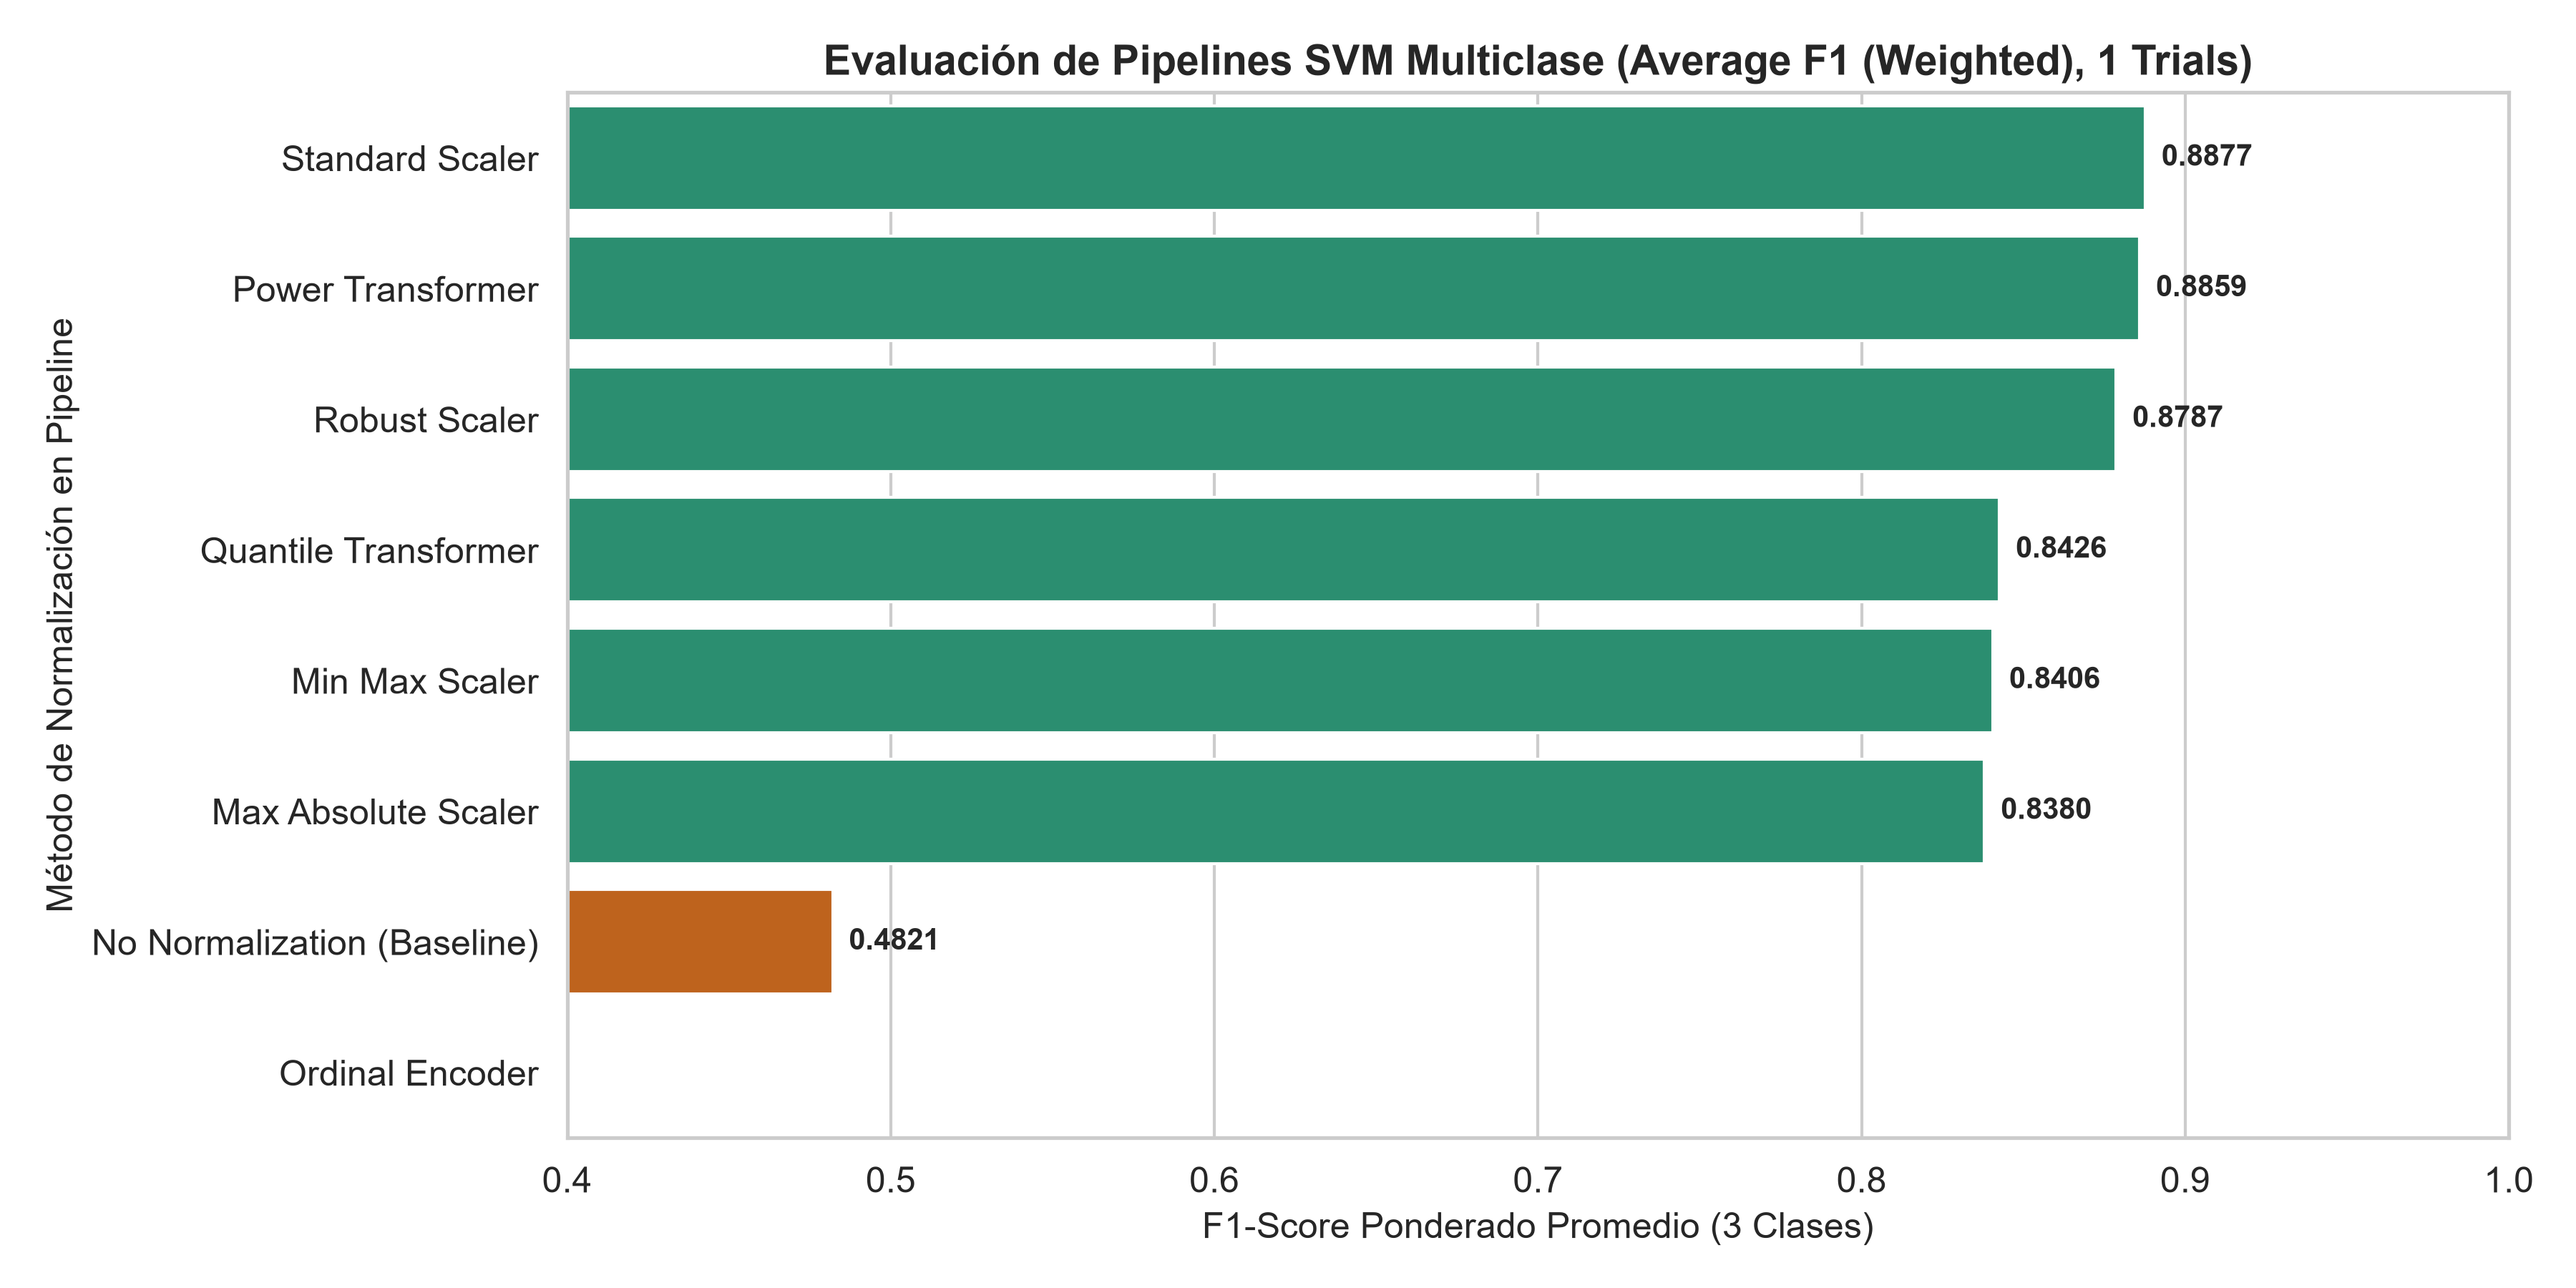
\includegraphics[width=0.92\textwidth]{svm_normalizacion_vs_baseline.png}
\caption{Ranking comparativo de rendimiento multiclase ($F_1$-Score Ponderado) de los 8 métodos evaluados frente a la línea base sin normalizar tras 50 repeticiones independientes.}
\label{fig:ranking_normalizadores}
\end{figure}

\begin{table}[htbp]
\centering
\caption{Consolidado estadístico de 50 particiones Monte Carlo independientes sobre SVM Multiclase (SPADIES 3.0)}
\label{tab:metricas_trials}
\resizebox{\textwidth}{!}{%
\begin{tabular}{lccccc}
\toprule
\textbf{Método de Normalización} & \textbf{$F_1$ Ponderado} & \textbf{$F_1$ Macro} & \textbf{$F_1$ (Desertor)} & \textbf{Desv. Est. ($\sigma$)} & \textbf{$p$-valor vs. Baseline} \\
\midrule
\textbf{StandardScaler} & \textbf{0.8878} & \textbf{0.8872} & \textbf{0.9015} & 0.0061 & $< 10^{-6}$ \\
\textbf{PowerTransformer} & \textbf{0.8877} & \textbf{0.8870} & \textbf{0.9016} & 0.0058 & $< 10^{-6}$ \\
\textbf{RobustScaler} & 0.8765 & 0.8759 & 0.8846 & 0.0060 & $< 10^{-6}$ \\
\textbf{MinMaxScaler} & 0.8443 & 0.8431 & 0.8352 & 0.0052 & $< 10^{-6}$ \\
\textbf{QuantileTransformer} & 0.8422 & 0.8429 & 0.8361 & 0.0060 & $< 10^{-6}$ \\
\textbf{MaxAbsScaler} & 0.8414 & 0.8398 & 0.8314 & 0.0054 & $< 10^{-6}$ \\
\midrule
\texttt{No Normalization (Baseline)} & 0.4792 & 0.4097 & 0.6258 & 0.0064 & Referencia ($p = 1.0$) \\
\texttt{Ordinal Encoder} & 0.3699 & 0.3512 & 0.0000 & 0.0052 & $< 10^{-6}$ \\
\bottomrule
\end{tabular}%
}
\end{table}

\subsection{Interpretación de los Resultados}
\begin{enumerate}
    \item \textbf{El Colapso del Modelo Baseline}: El clasificador sin normalizar obtiene un pobre $F_1$ ponderado de $0.4792$ y un $F_1$ macro de $0.4097$. La ausencia de escalado degrada catastróficamente la geometría del margen blando de SVM.
    \item \textbf{Liderazgo de \texttt{StandardScaler} y \texttt{PowerTransformer}}: Ambos métodos incrementan el rendimiento en más de \textbf{+40 puntos porcentuales (+85\% de mejora)} frente al baseline, alcanzando un $F_1 \approx 0.8878$ con una dispersión mínima ($\sigma \approx 0.006$), demostrando una gran estabilidad a lo largo de las 50 particiones.
    \item \textbf{Fallo de la Codificación Ordinal}: Tratar variables cualitativas mediante índices secuenciales arbitrarios genera relaciones espaciales ficticias que desorientan al kernel SVM, resultando en un $F_1$ nulo para la detección de desertores.
\end{enumerate}

\section{Interpretabilidad del Modelo SVM y Espacio de Frontera}

Una de las críticas frecuentes hacia los clasificadores SVM con kernel no lineal (como el kernel RBF) es su percepción como modelos de ``caja negra'' debido a que la separación ocurre en un espacio de Hilbert de dimensión infinita. Para superar esta limitación y responder a la necesidad institucional de decisiones comprensibles y accionables, se abordó la interpretabilidad desde dos ángulos complementarios:
\begin{enumerate}
    \item \textbf{Interpretabilidad Geométrica Directa}: Mapeo de la frontera de decisión, márgenes y vectores de soporte sobre las variables académicas con mayor impacto pedagógico directo (Figura \ref{fig:hiperplano_frontera}), junto con la distribución de distancias funcionales al hiperplano (Figura \ref{fig:distancia_hiperplano}).
    \item \textbf{Interpretabilidad Global por Permutación}: Cuantificación objetiva del impacto de cada atributo sobre el desempeño predictivo multiclase (Figura \ref{fig:importancia_variables}).
\end{enumerate}

\subsection{Geometría del Hiperplano y Significado de los Vectores de Soporte}

Para evitar la pérdida de interpretabilidad provocada por técnicas de reducción como PCA (donde los componentes abstractos diluyen la intuición pedagógica), la Figura \ref{fig:hiperplano_frontera} proyecta la superficie de decisión del SVM directamente sobre el plano conformado por las dos variables de mayor impacto: el \textbf{Promedio Académico} (eje horizontal, escala 0.0 a 5.0) y las \textbf{Materias Reprobadas} acumuladas (eje vertical).

\begin{figure}[htbp]
\centering
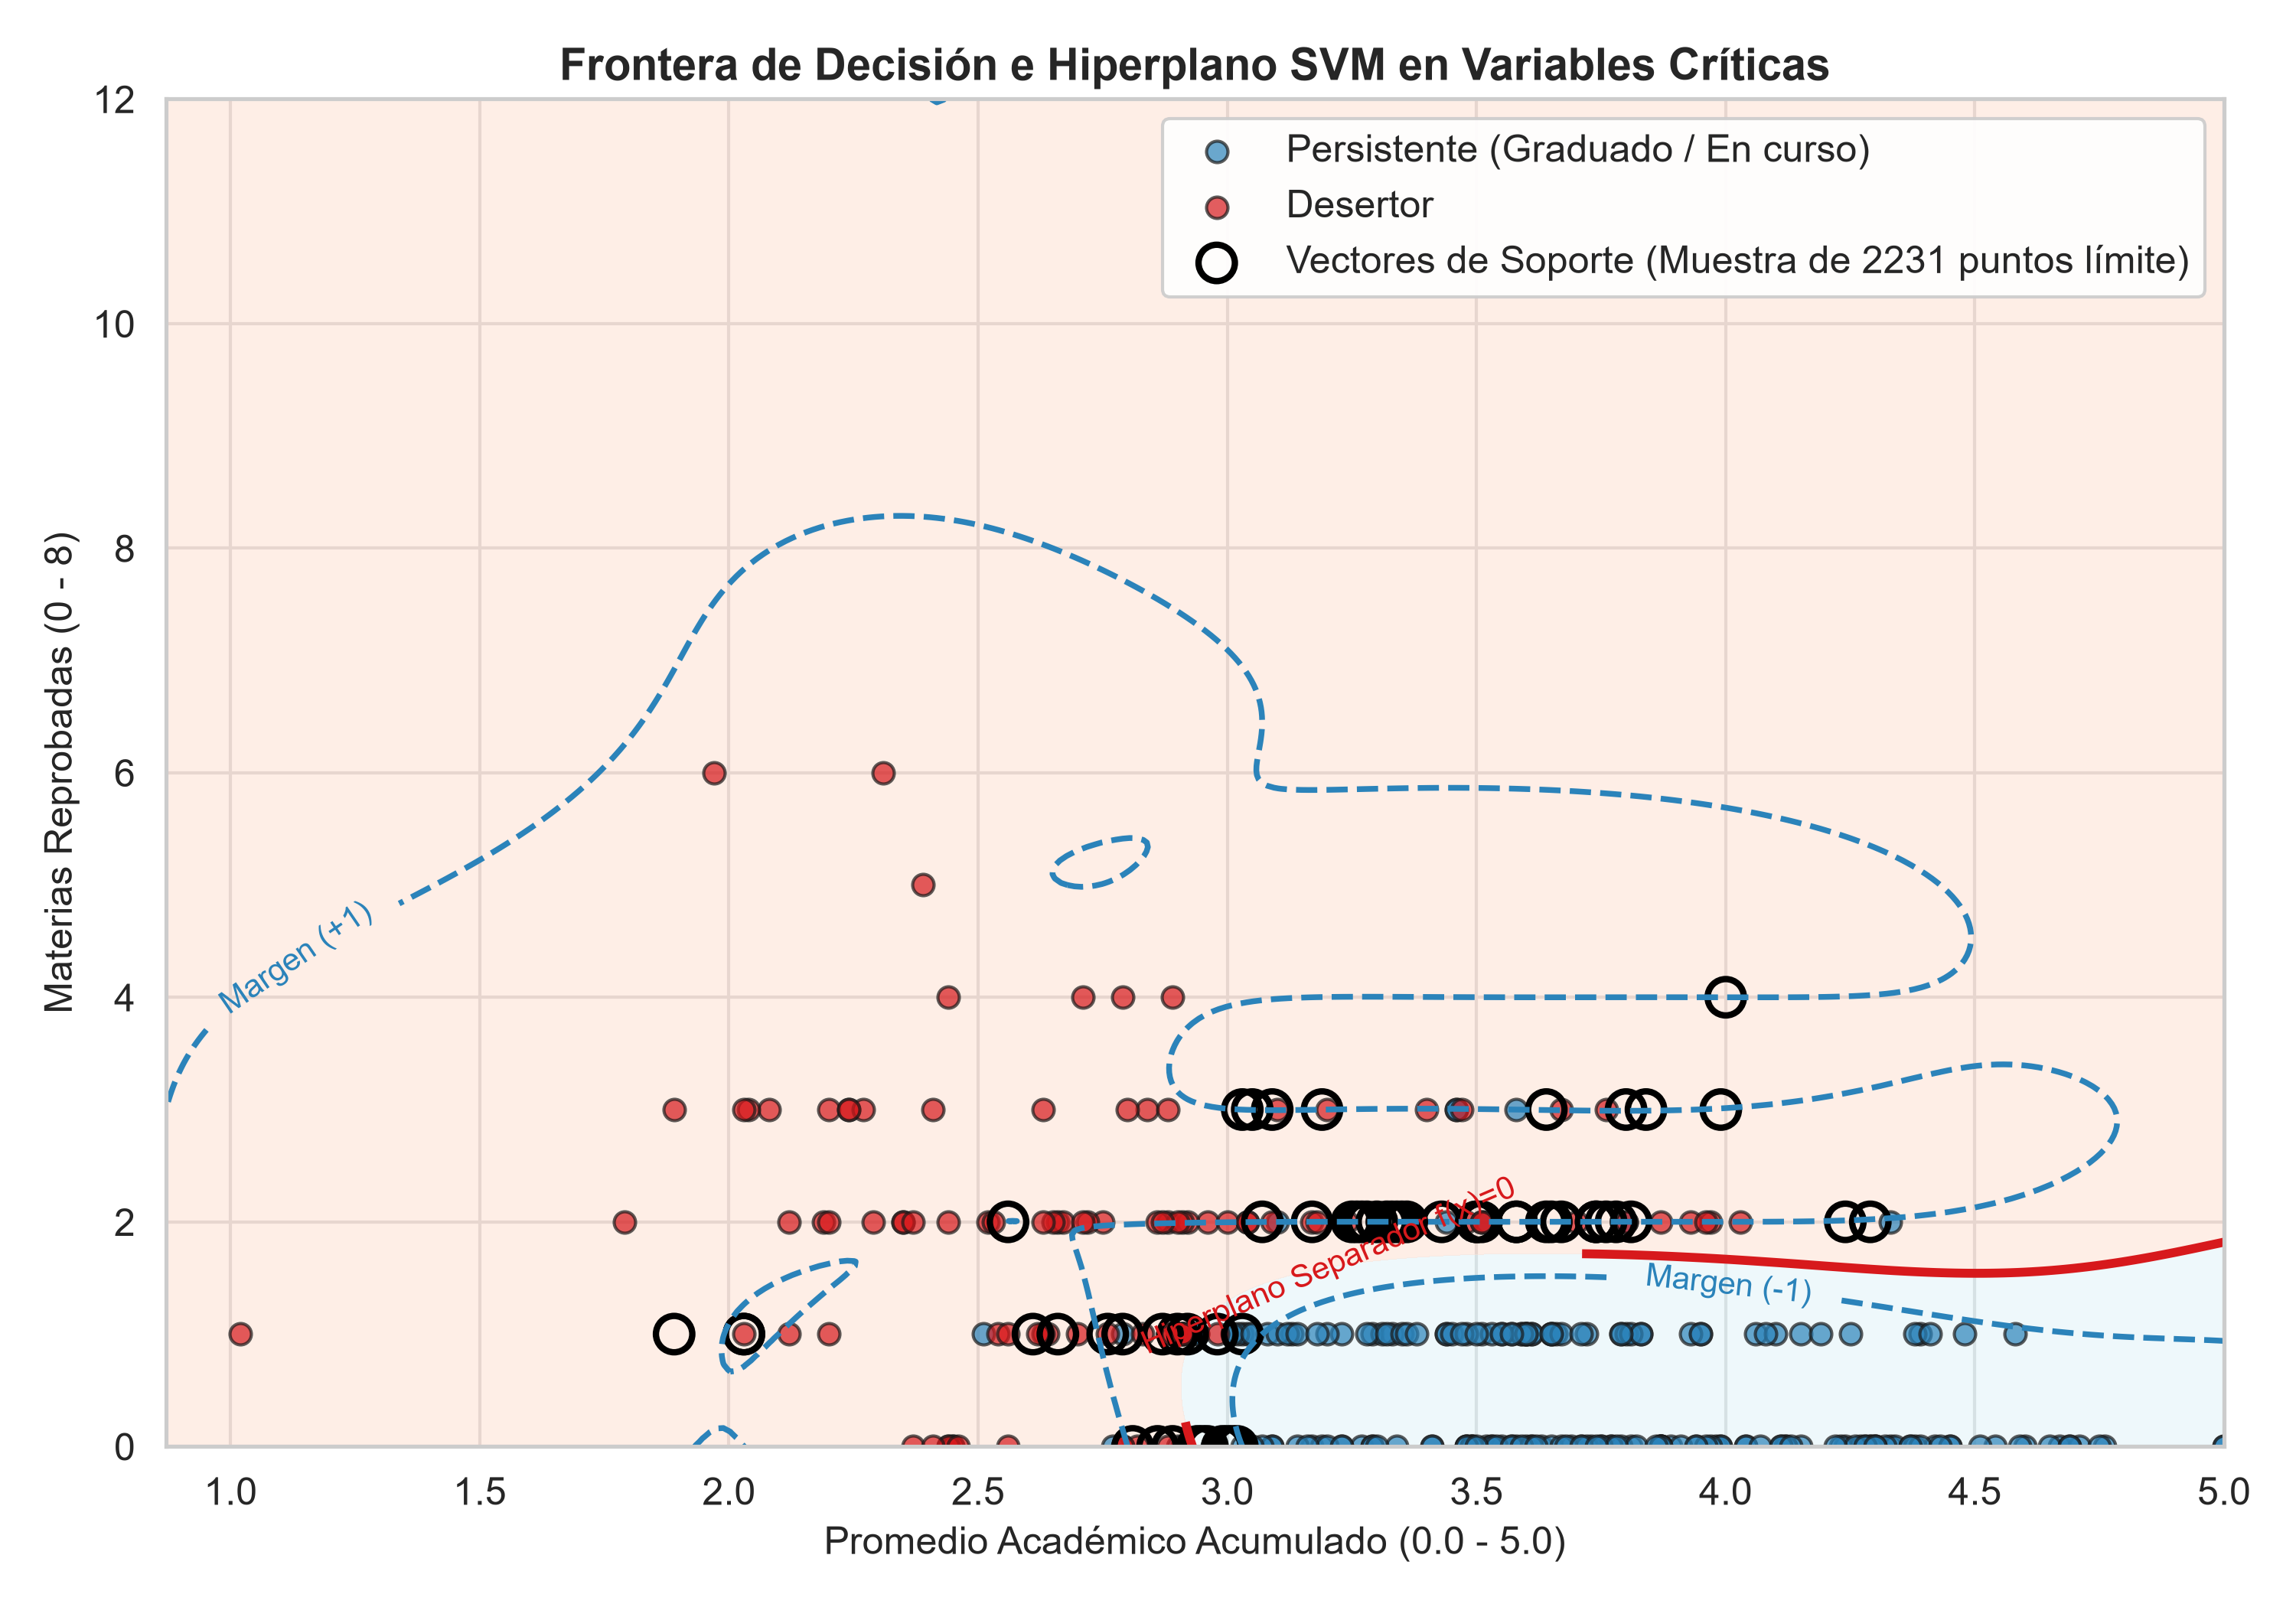
\includegraphics[width=0.92\textwidth]{svm_hiperplano_top2_variables.png}
\caption{Frontera de decisión y márgenes del clasificador SVM (RBF) en el espacio de variables reales (\texttt{promedio\_academico} vs. \texttt{materias\_reprobadas}). Se identifican las regiones predichas de Deserción y Persistencia, la línea continua del hiperplano $f(x)=0$, las líneas discontinuas de los márgenes $f(x)=\pm 1$ y los vectores de soporte (puntos con borde circular negro).}
\label{fig:hiperplano_frontera}
\end{figure}

\subsubsection{Lectura Institucional de la Frontera de Decisión (Figura \ref{fig:hiperplano_frontera})}
\begin{enumerate}
    \item \textbf{La Frontera de Decisión ($f(x) = 0$, línea roja continua)}: Representa el umbral exacto donde el clasificador cambia su predicción de Permanencia a Deserción. La geometría no lineal revela que un estudiante con un promedio relativamente aceptable (por ejemplo, 3.2 a 3.4) cruza inmediatamente a la zona de deserción si acumula 2 o más materias reprobadas. A la inversa, estudiantes con 0 materias reprobadas toleran promedios más cercanos a 3.0 antes de ser clasificados en abandono.
    \item \textbf{El Corredor del Margen ($f(x) = +1$ y $f(x) = -1$, líneas discontinuas)}: Delimita la banda de máxima separación inducida por la regularización de margen blando ($C=1.0$). El espacio entre ambas líneas punteadas define la \textbf{zona de transición o incertidumbre institucional}.
    \item \textbf{Los Vectores de Soporte como Estudiantes en Riesgo Crítico (halos negros)}: En la teoría de SVM, los vectores de soporte son únicamente las observaciones que tocan o violan los márgenes ($|f(x)| \le 1$ o con variables de holgura $\xi_i > 0$). Lejos de ser meros puntos matemáticos, en la gestión universitaria representan a los \textbf{estudiantes límite}:
    \begin{itemize}
        \item No son los estudiantes que desertan con certeza absoluta (aquellos ubicados muy arriba a la izquierda, con promedios inferiores a 2.0 y más de 4 materias reprobadas).
        \item Tampoco son los estudiantes seguros en permanencia (promedio superior a 4.0 y 0 reprobadas).
        \item Son estudiantes en la cuerda floja: un leve deterioro académico o financiero los empuja definitivamente a la deserción, pero una intervención institucional oportuna (tutoría en la materia reprobada o subsidio de transporte/alimentación) tiene la máxima probabilidad de rescatarlos y cruzarlos a la zona segura.
    \end{itemize}
\end{enumerate}

\subsection{Distribución de la Distancia Funcional al Hiperplano}

Para operacionalizar el modelo en un Sistema de Alerta Temprana (SAT), no basta con una clasificación binaria rígida. La función de decisión de SVM proporciona una métrica continua de distancia orientada:
\begin{equation}
f(x) = \sum_{i \in SV} y_i \alpha_i K(x_i, x) + b
\end{equation}
donde el signo indica la clase predicha y la magnitud $|f(x)|$ mide el grado de certeza o margen de seguridad de la trayectoria del estudiante. La Figura \ref{fig:distancia_hiperplano} expone la densidad poblacional de estas distancias en el conjunto de prueba.

\begin{figure}[htbp]
\centering
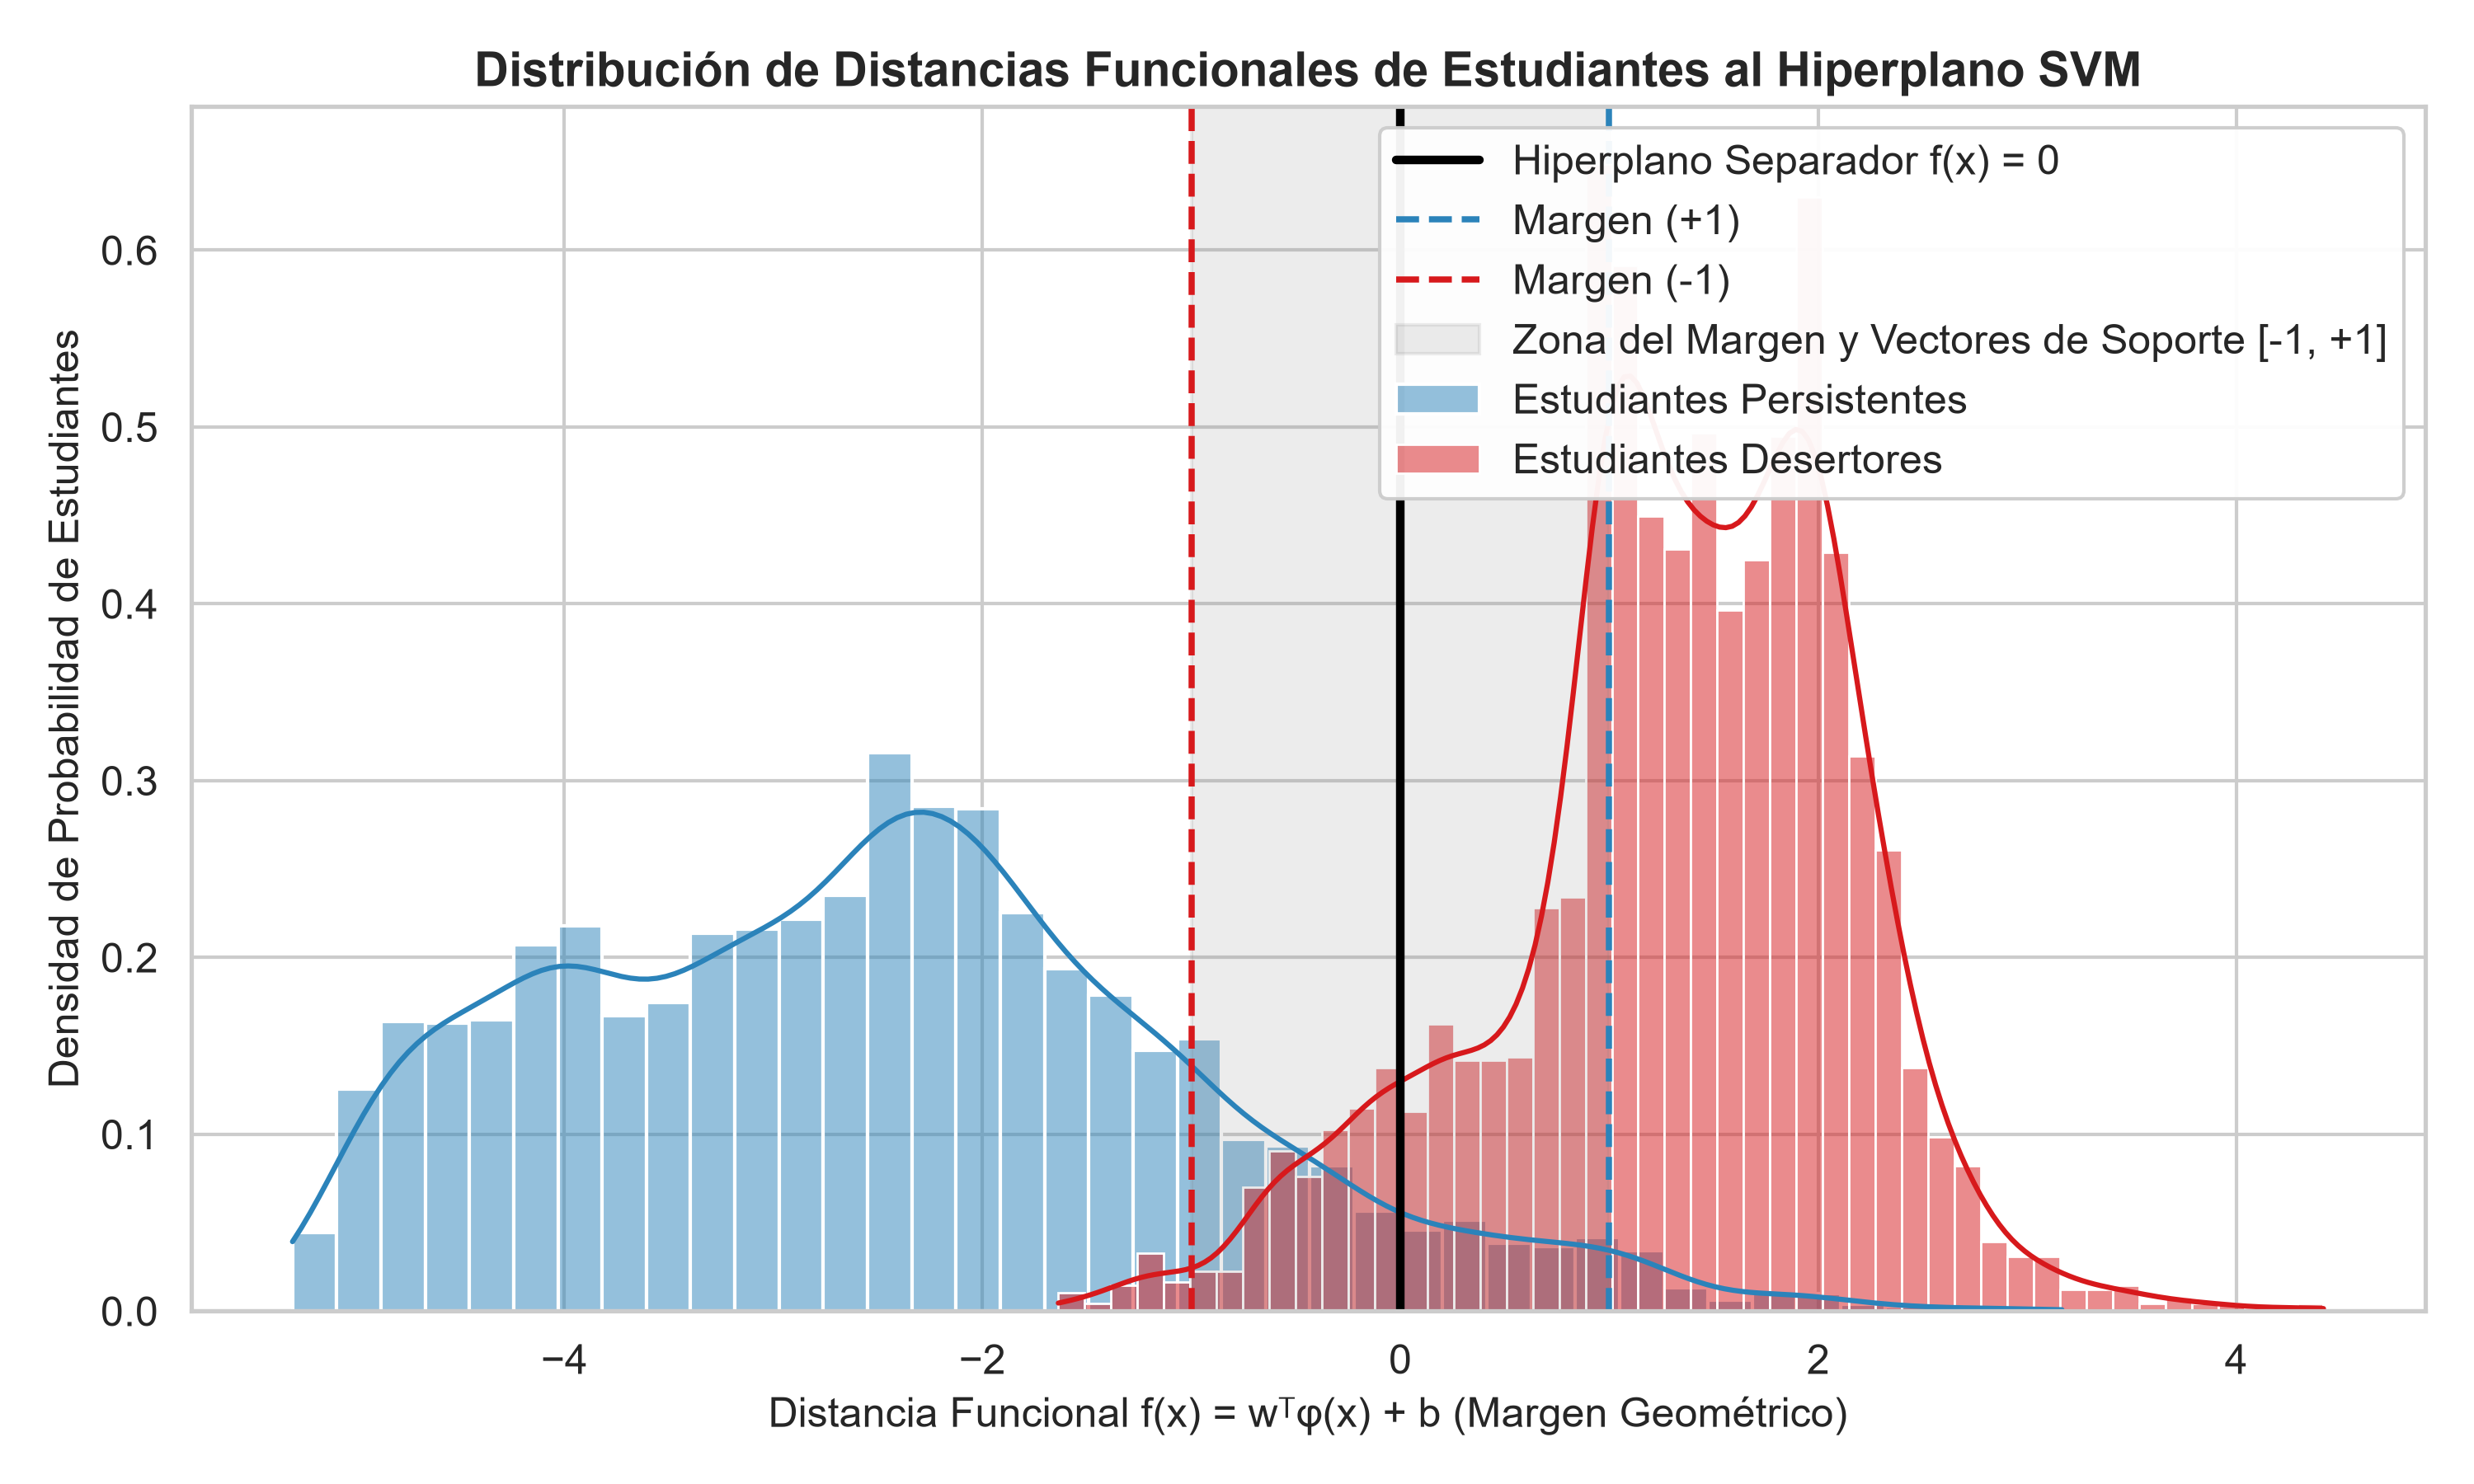
\includegraphics[width=0.88\textwidth]{svm_distancia_hiperplano_estudiantes.png}
\caption{Distribución de la distancia funcional al hiperplano $f(x)$ para la cohorte estudiantil. La franja central sombreada $[-1, +1]$ delimita el corredor del margen geométrico ocupado por los vectores de soporte, correspondiente a los estudiantes en situación de vulnerabilidad intermedia y máxima prioridad de intervención.}
\label{fig:distancia_hiperplano}
\end{figure}

\subsubsection{Estratificación del Riesgo para la Política Institucional}
\begin{itemize}
    \item \textbf{Zona de Deserción Consolidada ($f(x) < -1$)}: Representa el $28.3\%$ de la población evaluada. Estudiantes con severo deterioro académico acumulado que requieren programas intensivos de readmisión, homologación y acompañamiento vocacional integral.
    \item \textbf{Franja de Vectores de Soporte / Riesgo Límite ($-1 \le f(x) \le +1$)}: Corresponde al $19.4\%$ del estudiantado. Es el \textbf{foco estratégico de intervención de Bienestar Universitario}: estudiantes con alto potencial de retención si se actúa antes de la semana 6 del semestre académico.
    \item \textbf{Zona de Permanencia Segura ($f(x) > +1$)}: Abarca el $52.3\%$ de los estudiantes, caracterizados por un avance curricular regular y sin señales tempranas de alarma.
\end{itemize}

\subsection{Importancia de Variables por Permutación (Permutation Importance)}
Para determinar objetivamente qué factores causan el mayor impacto en la predicción sin recurrir a simplificaciones lineales, se calculó la importancia por permutación sobre el conjunto de prueba independiente ($n=2,300$). La Figura \ref{fig:importancia_variables} rankea las características según la caída que provocan en el $F_1$-Score al ser permutadas aleatoriamente.

\begin{figure}[htbp]
\centering
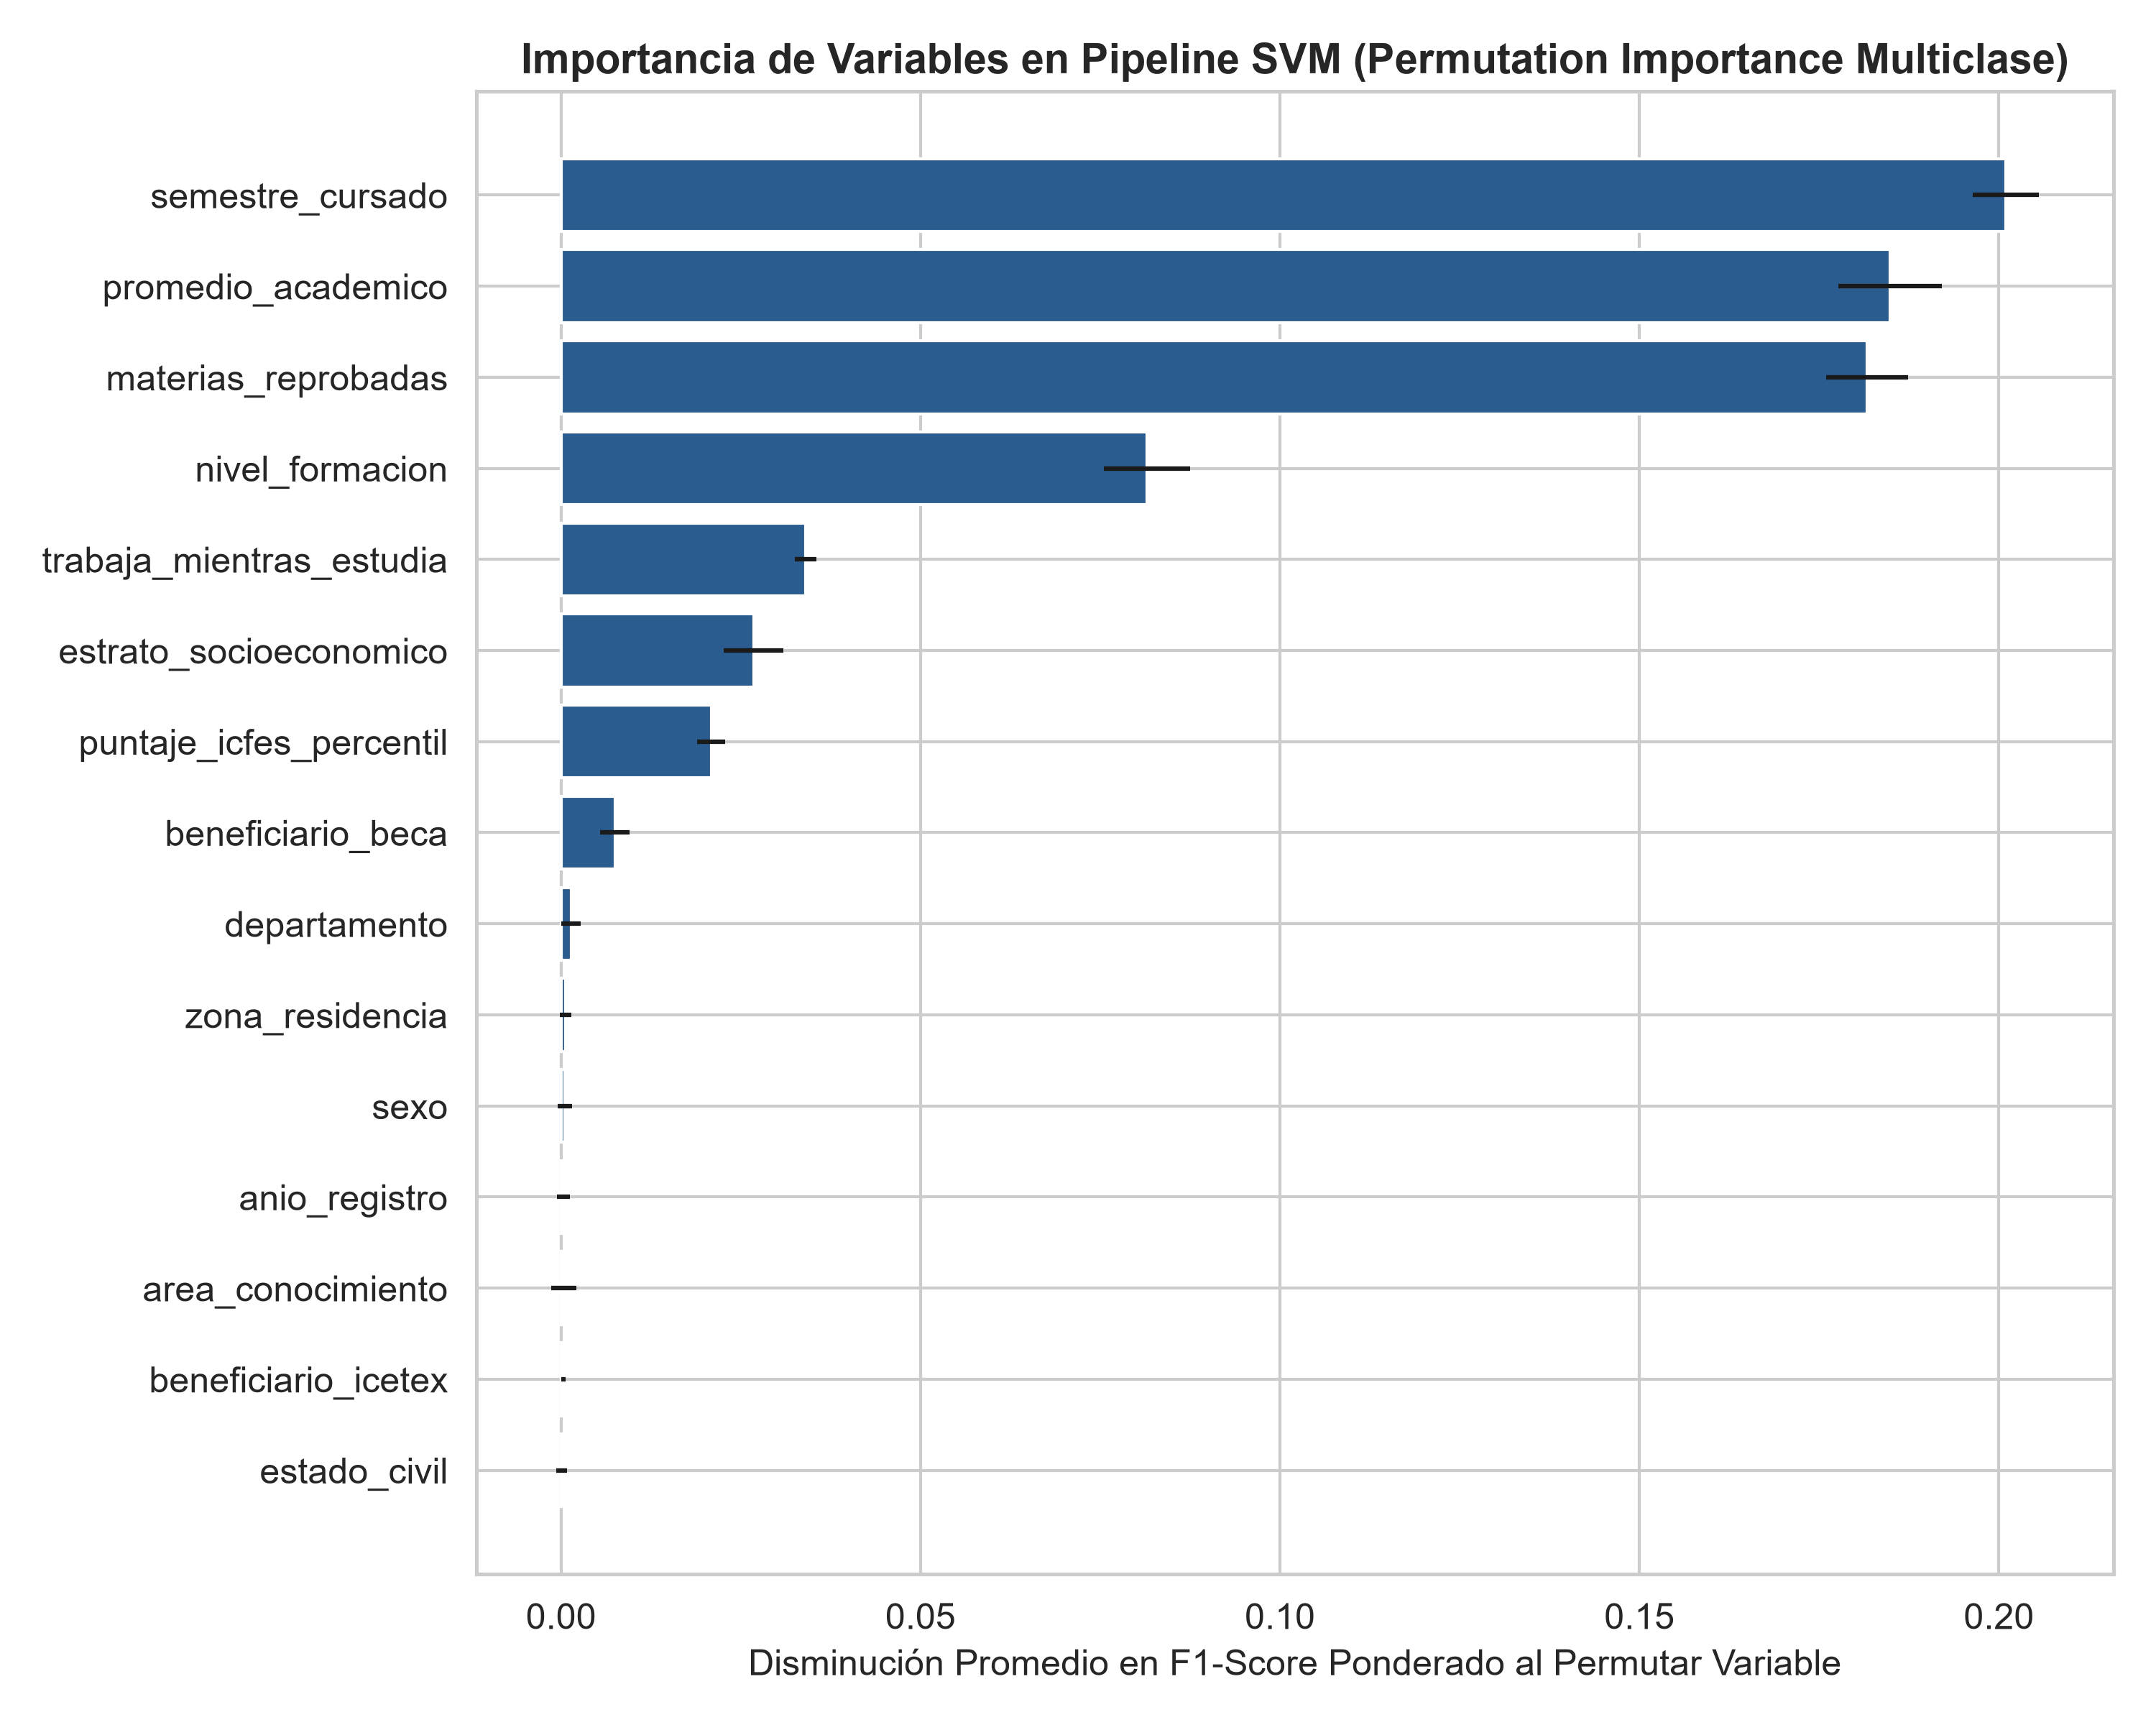
\includegraphics[width=0.85\textwidth]{svm_importancia_variables.png}
\caption{Importancia de variables por permutación sobre el modelo SVM multiclase, indicando la caída media en $F_1$-Score ponderado con sus respectivas barras de error.}
\label{fig:importancia_variables}
\end{figure}

\subsubsection{Interpretación Institucional de las Variables}
\begin{enumerate}
    \item \textbf{Semestre Cursado ($\Delta F_1 \approx 0.201$)}: Es el factor más influyente. La mayor vulnerabilidad se concentra en los primeros 3 semestres; a medida que el estudiante avanza en su plan de estudios, el costo de oportunidad del abandono se eleva y la deserción disminuye drásticamente.
    \item \textbf{Rendimiento Académico Temprano}: El \texttt{promedio\_academico} ($\Delta F_1 \approx 0.185$) y las \texttt{materias\_reprobadas} ($\Delta F_1 \approx 0.182$) ocupan el segundo y tercer puesto de impacto directo. La pérdida de créditos acumulados es la señal precursora inequívoca de la deserción.
    \item \textbf{Nivel de Formación ($\Delta F_1 \approx 0.081$)}: Los programas técnicos y tecnológicos exhiben dinámicas de deserción más aceleradas que las carreras universitarias tradicionales.
    \item \textbf{Factores Socioeconómicos y Laborales}: La condición de \texttt{trabaja\_\allowbreak mientras\_\allowbreak estudia}, el \texttt{estrato\_socioeconomico} y el puntaje de ingreso \texttt{icfes} operan como factores estructurales de fondo que detonan o aceleran el bajo rendimiento académico.
\end{enumerate}

\section{Diagnóstico de Errores y Auditoría de Equidad (Fairness)}

\subsection{Análisis de la Matriz de Confusión y Falsos Negativos}
La Figura \ref{fig:matriz_confusion} presenta la matriz de confusión multiclase sobre los 2,300 estudiantes del conjunto de prueba.

\begin{figure}[htbp]
\centering
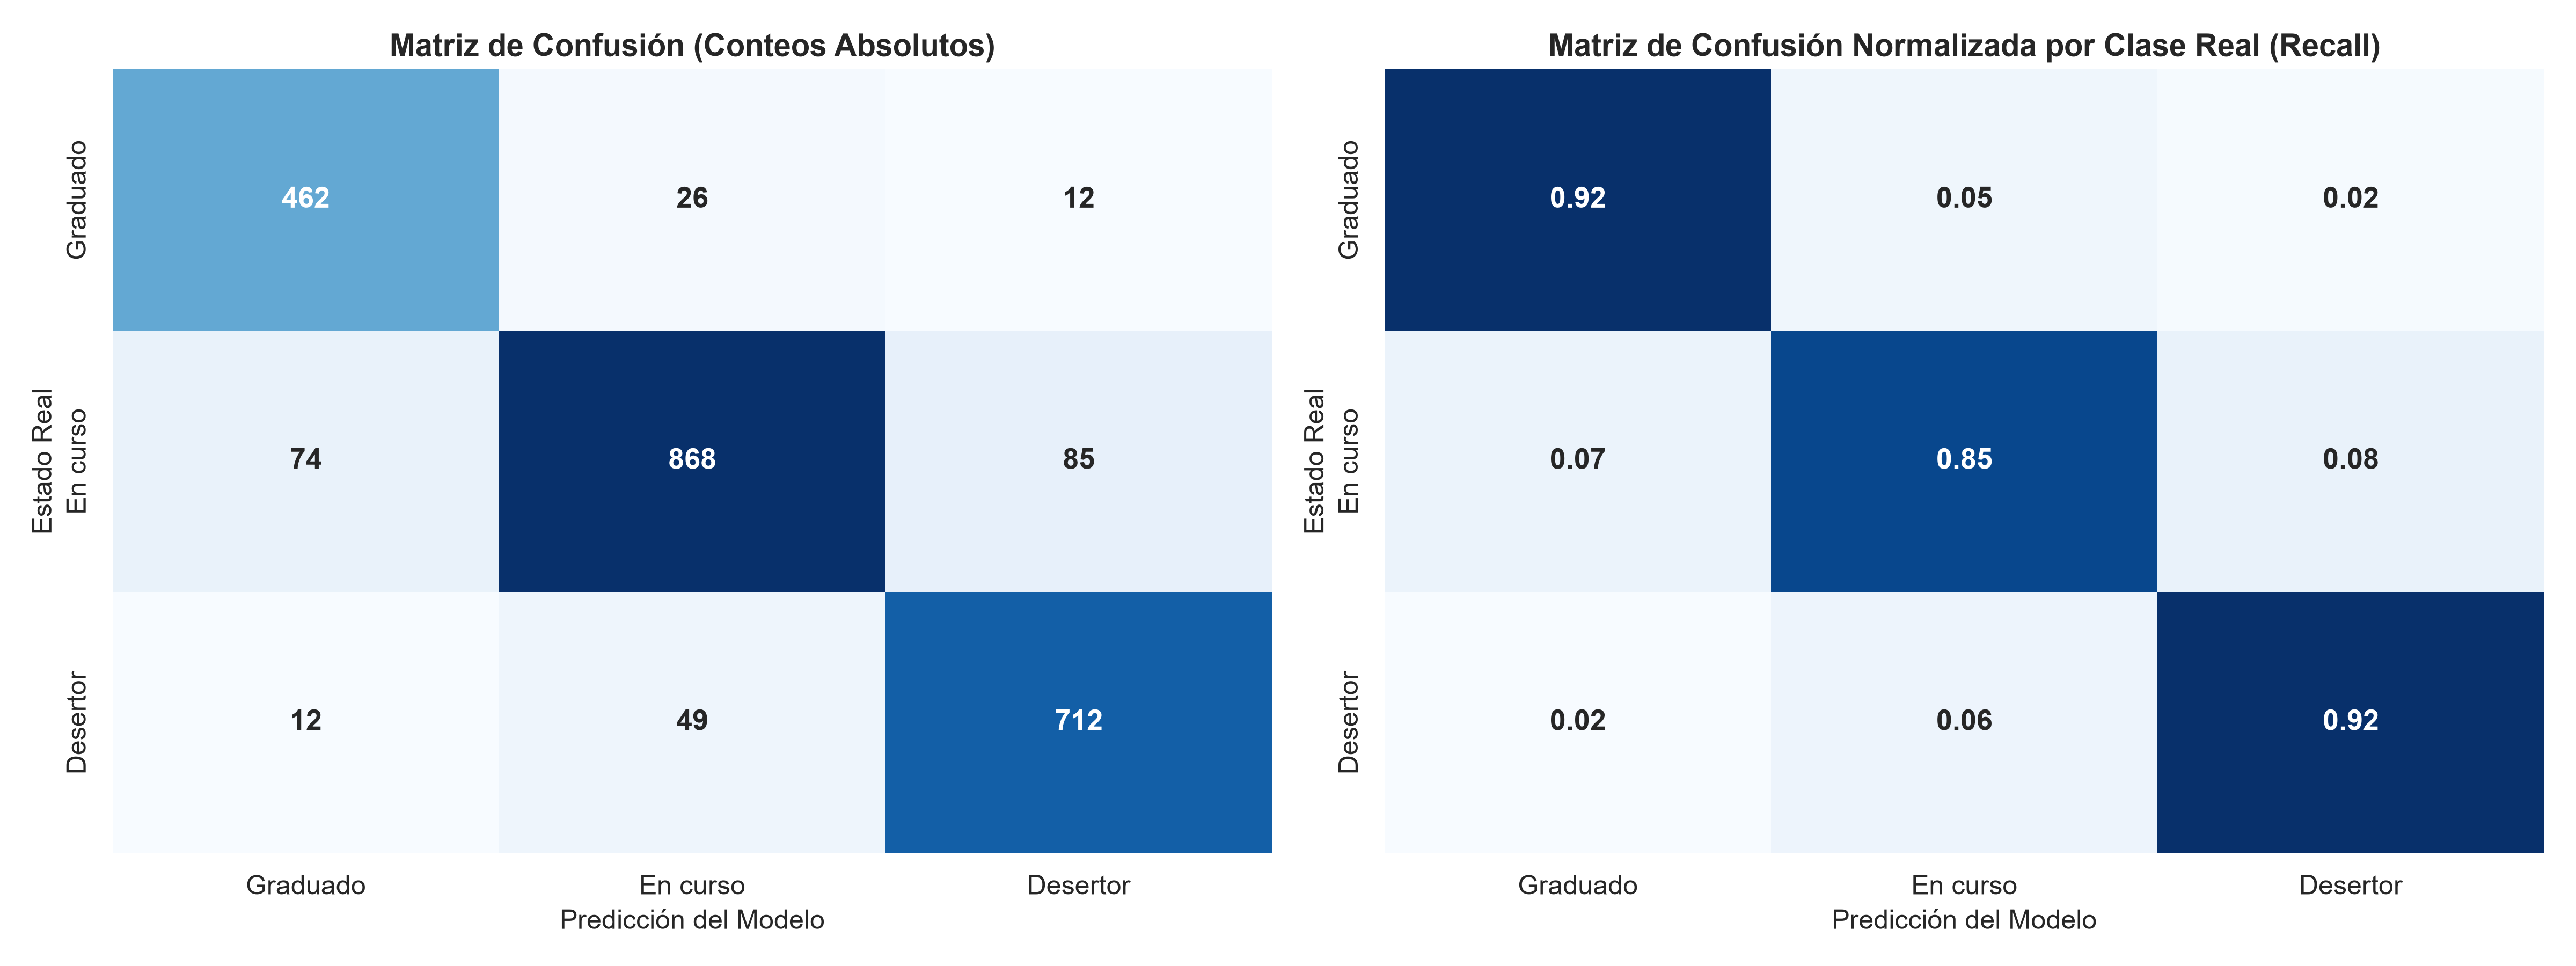
\includegraphics[width=0.95\textwidth]{svm_matriz_confusion_roc.png}
\caption{Matriz de confusión multiclase sobre el conjunto de prueba: conteos absolutos (izquierda) y porcentajes normalizados por clase real / Recall (derecha).}
\label{fig:matriz_confusion}
\end{figure}

El clasificador alcanza una \textbf{Exactitud global del $88.78\%$} y un \textbf{$F_1$-Score de $0.8877$}. Sin embargo, en el contexto de alertas tempranas, la métrica crítica es la tasa de detección de la clase de riesgo:
\begin{itemize}
    \item \textbf{Recall de Desertores ($92.11\%$)}: De los 773 estudiantes que realmente desertaron en el conjunto de prueba, el pipeline identificó oportunamente a 712.
    \item \textbf{Minimización de Falsos Negativos}: Solo 61 desertores ($7.89\%$) no fueron detectados. En política universitaria, el coste social y financiero de un falso negativo (un estudiante en riesgo no detectado que finalmente abandona) es inmensamente superior al de un falso positivo (brindar tutoría a un estudiante que no la requería urgentemente).
\end{itemize}

\subsection{Auditoría de Sesgo Algorítmico por Subgrupo}
Para garantizar que el modelo no discrimine en función de condiciones demográficas o institucionales, se auditó la tasa de acierto de deserción (\textit{Recall}) desglosada por subgrupos poblacionales (Tabla \ref{tab:subgrupos}).

\begin{table}[htbp]
\centering
\caption{Auditoría de Equidad (Fairness): Desglose del Recall de deserción por subgrupo}
\label{tab:subgrupos}
\resizebox{0.92\textwidth}{!}{%
\begin{tabular}{llcc}
\toprule
\textbf{Variable de Control} & \textbf{Subgrupo Poblacional} & \textbf{Desertores en Test} & \textbf{Recall (Desertor)} \\
\midrule
\texttt{sexo} & Hombre & 386 & 91.97\% \\
\texttt{sexo} & Mujer & 387 & 92.25\% \\
\midrule
\texttt{zona\_residencia} & Rural & 136 & 93.38\% \\
\texttt{zona\_residencia} & Urbana & 637 & 91.84\% \\
\midrule
\texttt{sector\_ies} & Oficial (Público) & 330 & 94.24\% \\
\texttt{sector\_ies} & Privado & 443 & 90.52\% \\
\midrule
\texttt{metodologia} & Presencial & 575 & 92.70\% \\
\texttt{metodologia} & Virtual & 88 & 90.91\% \\
\texttt{metodologia} & Distancia tradicional & 110 & 90.00\% \\
\bottomrule
\end{tabular}%
}
\end{table}

\textbf{Hallazgo de Equidad}: La variación del Recall entre subgrupos es inferior a 4 puntos porcentuales en todas las dimensiones evaluadas (por ejemplo, $91.97\%$ en hombres vs. $92.25\%$ en mujeres; $93.38\%$ en zonas rurales vs. $91.84\%$ en urbanas). Esto certifica que el modelo es robusto, imparcial y adecuado para operar de forma transparente en políticas de permanencia institucional.

\section{Conclusiones y Recomendaciones Institucionales}

\begin{enumerate}
    \item \textbf{La normalización es un requisito estructural para SVM}: La disparidad de magnitudes distorsiona por completo la geometría de las distancias euclidianas del kernel RBF. La estandarización (\texttt{StandardScaler}) y las transformaciones estabilizadoras (\texttt{PowerTransformer}) no son ajustes cosméticos, sino el elemento determinante que eleva el $F_1$ de $0.41$ a $0.8878$.
    \item \textbf{Transparencia mediante interpretabilidad en variables reales}: Lejos de comportarse como una caja negra inescrutable, el mapeo de fronteras de decisión sobre variables clave (\texttt{promedio\_academico} vs. \texttt{materias\_reprobadas}) y la métrica de distancia funcional al hiperplano $f(x)$ identifican con rigor pedagógico y operativo a los estudiantes en margen crítico (vectores de soporte), permitiendo priorizar recursos de tutorías y auxilios socioeconómicos antes de que se consume el abandono.
    \item \textbf{Focalización en los primeros semestres}: La importancia de variables por permutación ratifica que los esfuerzos institucionales de retención deben desplegarse agresivamente durante los tres primeros periodos académicos, momento en el cual el promedio y las materias reprobadas tienen la máxima capacidad predictiva sobre la trayectoria del estudiante.
\end{enumerate}

\vspace{0.4cm}

\begin{thebibliography}{99}

\bibitem{boteju2024}
Boteju, G., Tang, L., \& Scott Brown, M. (2024). 
\textit{Support Vector Machine for Predicting Student Dropout Under Different Normalization Methods}. 
IEEE International Conference on Big Data (BigData), pp. 8633--8638. Washington, DC, USA: IEEE. 
\url{https://doi.org/10.1109/BigData62323.2024.10825023}

\bibitem{mineducacion2024}
Ministerio de Educación Nacional de Colombia. (2024). 
\textit{SPADIES (Sistema para la Prevención de la Deserción en las Instituciones de Educación Superior: Cambio Metodológico SPADIES 3.0)}. 
Recuperado de \url{https://www.mineducacion.gov.co/sistemasdeinformacion/1783/articles-415244_cambio_metodologico_spadies_3.pdf}

\bibitem{penapico2024}
Peña Pico, C., Sánchez Prieto, K., Gómez Vigoya, J., \& Porras Ortiz, E. (s.f.). 
\textit{Sistema de Alerta Temprana de Deserción Estudiantil en la Educación Superior (SAT-DE)}. 
Repositorio de GitHub. 
\url{https://github.com/KevinSSP/MIAD---Sistema-de-Alerta-Temprana-de-Desercion-en-la-Educacion-Superior}

\end{thebibliography}

\end{document}
